%%%%%%%%%%%%%%%%%%%%%%%%%%%%%%%%%%%%%%%%%%%%%%%%%%%%%%%%%%%%%%%%%%%%%%%%
%                                                                      %
%     File: Thesis_Results.tex                                         %
%     Tex Master: Thesis.tex                                           %
%                                                                      %
%     Author: Andre C. Marta                                           %
%     Last modified :  2 Jul 2015                                      %
%                                                                      %
%%%%%%%%%%%%%%%%%%%%%%%%%%%%%%%%%%%%%%%%%%%%%%%%%%%%%%%%%%%%%%%%%%%%%%%%

\chapter{Results}
\label{chapter:results}

In this chapter we describe the main results of the search for $hh\rightarrow b\overline{b}b\overline{b}$ at the FCC-hh (section \ref{sec:dihiggs_FCC}). In section \ref{sec:gran_studies} we show how the significance of the analysis varies as a function of the granularity of the HCAL and/or the detector configuration. We also compare the results obtained using particle flow and pure calorimeter jets.

\section{Di-Higgs discovery potential at the FCC-hh}
\label{sec:dihiggs_FCC}

The event selection of the optimized analysis for the search for $hh\rightarrow b\overline{b}b\overline{b}$ at the FCC-hh with the baseline detector design is summarized in tables \ref{table:cutflow_sig_FCC} and \ref{table:cutflow_bkg_FCC} for the signal samples (SM, DM mediator and type II 2HDM) and for the background samples ($4b+j$, $jj+0/1/2 j$ and $t\overline{t}$), respectively.

From table \ref{table:cutflow_sig_FCC}, we see that for the BSM models the signal efficiency is higher than for the SM. It varies from $0.446\%$ for the SM, to $0.487\%$ for the DM mediator model and to $1.666\%$ for the type II 2HDM. This is due to the existence of heavy new particles in the BSM models that lead to the production of highly boosted SM Higgs pairs.

Considering the SM production of Higgs pairs, the achieved significance is
\begin{equation}
	S/\sqrt{B}=8.8\pm 1.6~\text{(stat.)}~^{+4.1}_{-3.0}~\text{(sys.)}\quad \left(2.8\pm 0.5~\text{(stat.)}~^{+1.3}_{-1.0}~\text{(sys.)}\right)
\end{equation}
for an integrated luminosity of $30~(3)~\text{ab}^{-1}$. For $\mathcal{L}=30~\text{ab}^{-1}$, the significance is above the $5\sigma$ threshold. This result indicates that with the entire dataset that is expected to be accumulated by the FCC-hh detector it should be possible to observe the production of Higgs pairs.

For the signal model that includes a $1$ TeV dark matter mediator that can decay to pairs of SM Higgs bosons the achieve significance is $2.3\pm0.4~\text{(stat.)}~^{+1.1}_{-0.8}~\text{(sys.)}~\left(0.73\pm0.13~\text{(stat.)}~^{+0.34}_{-0.25}~\text{(sys.)}\right)$ for an integrated luminosity of $30~(3)~\text{ab}^{-1}$. The significance is well bellow the $3\sigma$ threshold for both luminosities. Therefore, we do not expect to be able to detect or exclude this signal at the FCC-hh. In this model, the coupling of the DM mediator to the Higgs pairs is small which means that the contribution from the box diagram dominates over the resonant production (s-channel diagram), just like in the SM. In addition, the cross section is smaller than for the SM process which leads to a smaller significance even though the efficiency is higher.

For the type II 2HDM the achieved significance is
\begin{equation}
	S/\sqrt{B}=16.9\pm 3.0~\text{(stat.)}~^{+8.0}_{-5.9}~\text{(sys.)}~\left(5.4\pm 0.9~\text{(stat.)}~^{+2.5}_{-1.9}~\text{(sys.)}\right)
\end{equation}
for an integrated luminosity of $30~(3)~\text{ab}^{-1}$. These results indicate that the contribution of this model to the production of Higgs pairs can be observed (or excluded) at the FCC-hh. The high efficiency of this signal sample through the cuts, reflected in the high significance that is achieved, make it a very exciting and achievable benchmark. 

%\begin{table}
%	\begin{tabular}{lcccccccccc}
%		\toprule 
%		\textbf{Selection} & SM & $\epsilon(\%)$ & 2HDM & $\epsilon(\%)$ & 4b+j & $\epsilon(\%)$& jj+0/1/2 j &$\epsilon(\%)$& $t\overline{t}$+0/1/2 j & $\epsilon(\%)$\\
%		\midrule
%		Gen level & $3.46\text{e}7$ & $100$& $5.55\text{e}7$ & $100$&$4.90\text{e}10$ & $100$&$5.47\text{e}14$ &$100$ &$2.25\text{e}12$&$100$\\
%		\rowcolor{black!10}N(b-tags)$\geq4$ & $3.20\text{e}7$& $92.5$ & $5.09\text{e}7$& $91.8$& $3.72\text{e}10$ & $75.8$ &$2.17\text{e}13$ & $3.963$&$1.20\text{e}12$& $53.5$\\
%		$p_T(j_1,j_2)\geq200$ GeV & $5.75\text{e}6$ & $16.6$ & $1.70\text{e}7$& $30.6$&$8.73\text{e}9$ & $17.8$& $4.06\text{e}12$ &$0.74$ &$2.38\text{e}10$ & $1.06$\\
%		\rowcolor{black!10}$p_T(j_1)\geq 400$ GeV & $2.99\text{e}6$ & $8.623$ & $1.01\text{e}7$& $18.2$&$3.44\text{e}9$ & $7.0$ &$1.00\text{e}12$ & $0.18$ &$1.00\text{e}10$& $0.446$\\
%		$p_T(j_2)\geq 350$ GeV & $1.98\text{e}6$ & $5.7$ & $6.22\text{e}6$& $11.2$ &$1.93\text{e}9$ &$3.9$ &$6.61\text{e}11$ &$0.121$ &$5.92\text{e}9$& $0.263$\\
%		\rowcolor{black!10}$p_T(j_1+j_2)\geq 100$ GeV & $1.61\text{e}6$& $4.648$& $4.53\text{e}6$& $8.16$&$1.62\text{e}9$& $3.3$&$3.80\text{e}11$ & $0.07$ & $5.03\text{e}9$& $0.223$\\
%		$\tau_{21}(j_1,j_2)<0.55$ & $5.91\text{e}5$ & $1.7$ &$1.85\text{e}6$ &$3.3$&$2.65\text{e}8$ & $0.54$ & $2.95\text{e}10$ & $0.005$ & $1.56\text{e}9$ & $0.069$\\
%		\rowcolor{black!10}$FW2(j_1)>0.2$ &$4.44\text{e}5$ & $1.28$& $1.50\text{e}6$& $2.7$&$1.57\text{e}8$ & $ 0.32$&$1.78\text{e}10$ & $0.003$& $4.41\text{e}8$& $0.020$\\
%		$100<M_{SD}(j1,j2)<135$ GeV & $1.46\text{e}5$&$0.422$ &$6.07\text{e}5$ & $1.09$& $6.66\text{e}6$& $0.0136$ & $4.38\text{e}8$ & $0.00008$ & $1.75\text{e}7$& $0.00078$\\
%		\bottomrule
%	\end{tabular}
%	\caption{FCC default HCAL. Entries normalized to $\mathcal{L}=30~\text{ab}^{-1}$}
%\end{table}

\begin{table}
	\centering
	\caption{Cumulative efficiency, in percentage, of each event selection criterion for the signal samples (SM and 2HDM). The absolute value of expected events after some key selection cuts is shown in curved brackets. The number of expected events is normalized to $\mathcal{L}=30~\text{ab}^{-1}$. The double horizontal line marks the pre-selection cuts. These results were obtained using the FCC-hh baseline detector design, as implemented in Delphes by the FCC-hh study group.}
	\label{table:cutflow_sig_FCC}
	\begin{tabular}{lccc}
		\toprule 
		\textbf{Selection [FCC-hh]} & SM  & DM mediator &2HDM type II\\
		\midrule
		\multirow{2}{*}{Gen level} & $100$ & $100$ &$100$ \\
		&  $(2704\pm12)\times 10^3$ & $(65400\pm29)\times 10^2$ & $(13977\pm7)\times 10^3$ \\
		\rowcolor{black!7}N(b-tags)$\geq4$ & $92.488$ & $92.593$ &$93.430$\\
		\multirow{2}{*}{$p_T(j_1,j_2)\geq200$ GeV} & $16.602$ & $17.033$ &$33.975$ \\ 
		& $(4490\pm5)\times 10^3$ & $(11140\pm12)\times 10^2$ & $4734\pm4\times 10^3$\\
		\midrule \midrule
		\rowcolor{black!7}$p_T(j_1)\geq 300$ GeV & $13.521$ & $14.007$ &$20.869$\\ 
		$p_T(j_1+j_2)\geq 100$ GeV & $10.933$ &$11.301$&  $22.863$ \\
		\rowcolor{black!7}$\tau_{21}(j_1,j_2)<0.4$ & $1.309$&$1.410$ &$3.952$\\
		$|\Delta \eta (hh)|<1.5$& $1.071$& $1.154$& $3.479$\\
		\rowcolor{black!7}$FW2(j_1)>0.2$ & $0.989$&$1.064$& $3.276$\\
		\multirow{2}{*}{$(100<M_{SD}(j1,j2)<135)$ GeV} & $0.446$ & $0.487$&$1.666$\\
		&$(1207\pm8)\times 10^2$&$(3188\pm20)\times10$&$(2328\pm8)\times 10^2$\\
		\bottomrule
	\end{tabular}
\end{table}

\begin{table}
	\centering
	\caption{Cumulative efficiency, in percentage, of each event selection criterion for the background samples ($4b+j$, $jj+0/1/2 j$ and $t\overline{t}$+0/1/2 j). The absolute value of expected events after some key selection cuts is shown in curved brackets. The number of expected events is normalized to $\mathcal{L}=30~\text{ab}^{-1}$. The double horizontal line marks the pre-selection cuts. These results were obtained using the FCC-hh baseline detector design, as implemented in Delphes by the FCC-hh study group.}
	\label{table:cutflow_bkg_FCC}
	\begin{tabular}{lccc}
		\toprule 
		\textbf{Selection [FCC-hh]} & $4b+j$  & $jj+0/1/2 j$ & $t\overline{t}$ \\
		\midrule
		\multirow{2}{*}{Gen level} & $100$ & $100$ &$100$ \\
		&  $(49035\pm12)\times 10^6$ & $(54698\pm13)\times 10^{10}$ & $(22503\pm11)\times 10^8$ \\
		\rowcolor{black!7}N(b-tags)$\geq4$ & $75.819$ & $3.963$ &$53.495$\\
		\multirow{2}{*}{$p_T(j_1,j_2)\geq200$ GeV} & $17.811$ & $0.742$ &$1.056$ \\ 
		& $(8734\pm5)\times 10^6$ & $(4058\pm11)\times 10^9$ & $(2377\pm11)\times 10^7$\\
		\midrule \midrule
		\rowcolor{black!7}$p_T(j_1)\geq 300$ GeV & $12.744$ & $0.422$ &$0.718$\\ 
		$p_T(j_1+j_2)\geq 100$ GeV & $10.901$ &$0.245$&  $0.617$ \\
		\rowcolor{black!7}$\tau_{21}(j_1,j_2)<0.4$ & $0.256$&$0.002$ &$0.037$\\
		$|\Delta\eta(hh)|<1.5$& $0.130$& $0.001$& $0.024$\\
		\rowcolor{black!7}$FW2(j_1)>0.2$ & $0.105$&$0.001$& $0.014$\\
		\multirow{2}{*}{$(100<M_{SD}(j1,j2)<135)$ GeV} & $0.007$ & $0.00003$&$0.0007$\\
		&$(341\pm10)\times 10^4$&$(17\pm11)\times10^7$&$(149\pm28)\times 10^5$\\
		\bottomrule
	\end{tabular}
\end{table}

\subsection{Comparing with the ATLAS detector}

The event selection of the search for $hh\rightarrow b\overline{b}b\overline{b}$ with the ATLAS detector at a CM energy of $\sqrt{s}=100$ TeV is summarized in tables \ref{table:cutflow_sig_ATLAS} and \ref{table:cutflow_bkg_ATLAS} for the signal and background samples, respectively.

It is interesting to compare the results obtained with the FCC-hh default detector simulation with the ones obtained using the simulation of the ATLAS detector. These are summarized in table \ref{table:FCC_ATLAS_comp} in terms of the achieved significance for an integrated luminosity of $30~\text{ab}^{-1}$, for the different signal models.

For all the signal models, the significance increases approximately $50\%$ going from the ATLAS detector to the FCC-hh. This percentage is computed as $\left((S/\sqrt{B})_{\text{FCC}}-(S/\sqrt{B})_{\text{ATLAS}}\right)/(S/\sqrt{B})_{\text{ATLAS}}$. For the SM signal, nonetheless, using the ATLAS default detector configuration the achieved significance is already above $5\sigma$, for $\mathcal{L}=30~\text{ab}^{-1}$: $S/\sqrt{B}=5.7\pm 1.3 ~\text{(stat.)}~^{+3.1}_{-2.4}~\text{(sys.)}$. This indicates that the CM energy and the high luminosity are the key factors driving the discovery potential of the accelerator.

\begin{table}
	\centering
	\caption{Cumulative efficiency, in percentage, of each event selection criterion for the signal samples (SM and 2HDM). The absolute value of expected events after some key selection cuts is shown in curved brackets. The number of expected events is normalized to $\mathcal{L}=30~\text{ab}^{-1}$. The double horizontal line marks the pre-selection cuts. These results were obtained using the ATLAS detector design, as implemented in Delphes.}
	\label{table:cutflow_sig_ATLAS}
	\begin{tabular}{lccc}
		\toprule 
		\textbf{Selection [ATLAS]} & SM  & DM mediator &2HDM type II\\
		\midrule
		\multirow{2}{*}{Gen level} & $100$ & $100$ &$100$ \\
		&  $(27043\pm12)\times 10^3$ & $(65400\pm29)\times 10^2$ & $(13978\pm6) \times 10^3$  \\
		\rowcolor{black!7}N(b-tags)$\geq4$ & $88.690$ & $88.787$ & $89.643$\\
		\multirow{2}{*}{$p_T(j_1,j_2)\geq200$ GeV} & $15.533$ & $15.941$ $32.181$& \\ 
		& $(4201\pm5)\times 10^3$ & $(10426\pm12)\times 10^2$ & $(4498\pm4)\times 10^3$ \\
		\midrule \midrule
		\rowcolor{black!7}$p_T(j_1)\geq 300$ GeV & $12.599$ & $13.061$ & $29.141$\\ 
		$p_T(j_1+j_2)\geq 100$ GeV & $10.185$ &$10.526$& $21.523$  \\
		\rowcolor{black!7}$\tau_{21}(j_1,j_2)<0.4$ & $1.139$&$1.220$ & $3.411$\\
		$|\Delta\eta(hh)|<1.5$& $0.891$& $0.960$& $2.930$\\
		\rowcolor{black!7}$FW2(j_1)>0.2$ & $0.796$&$858$& $2.684$ \\
		\multirow{2}{*}{$(100<M_{SD}(j1,j2)<135)$ GeV} & $0.333$ & $0.360$& $1.266$\\
		&$(901\pm7)\times 10^2$&$(2358\pm18)\times10$& $(1770\pm7)\times 10^2$\\
		\bottomrule
	\end{tabular}
\end{table}

\begin{table}
	\centering
	\caption{Cumulative efficiency, in percentage, of each event selection criterion for the background samples ($4b+j$, $jj+0/1/2 j$ and $t\overline{t}$+0/1/2 j). The absolute value of expected events after some key selection cuts is shown in curved brackets. The number of expected events is normalized to $\mathcal{L}=30~\text{ab}^{-1}$. The double horizontal line marks the pre-selection cuts. These results were obtained using the ATLAS detector design, as implemented in Delphes.}
	\label{table:cutflow_bkg_ATLAS}
	\begin{tabular}{lccc}
		\toprule 
		\textbf{Selection [ATLAS]} & $4b+j$  & $jj+0/1/2 j$ & $t\overline{t}$ \\
		\midrule
		\multirow{2}{*}{Gen level} & $100$ & $100$ &$100$ \\
		&  $(49035\pm15)\times 10^6$ & $(54698\pm15)\times 10^{10}$ & $(22503\pm9)\times 10^8$ \\
		\rowcolor{black!7}N(b-tags)$\geq4$ & $71.617$ & $3.747$ &$51.782$\\
		\multirow{2}{*}{$p_T(j_1,j_2)\geq200$ GeV} & $16.299$ & $0.685$ &$0.985$ \\ 
		& $(7993\pm6)\times 10^6$ & $(379\pm11)\times 10^9$ & $(2215\pm9)\times 10^7$\\
		\midrule \midrule
		\rowcolor{black!7}$p_T(j_1)\geq 300$ GeV & $11.627$ & $0.390$ &$0.669$\\ 
		$p_T(j_1+j_2)\geq 100$ GeV & $9.932$ &$0.227$&  $0.574$ \\
		\rowcolor{black!7}
		$\tau_{21}(j_1,j_2)<0.4$ & $0.234$&$0.003$ &$0.031$\\
		$|\Delta\eta(hh)|<1.5$& $0.113$& $0.001$& $0.019$\\
		\rowcolor{black!7}$FW2(j_1)>0.2$ & $0.082$&$0.001$& $0.010$\\
		\multirow{2}{*}{$(100<M_{SD}(j1,j2)<135)$ GeV} & $0.005$ & $0.00004$&$0.0007$\\
		&$(253\pm11)\times 10^4$&$(23\pm15)\times10^7$&$(160\pm24)\times 10^5$\\
		\bottomrule
	\end{tabular}
	
\end{table}

\begin{table}
	\centering
	\caption{Significances achieved with the ATLAS and FCC-hh detector configurations for $\mathcal{L}=30~\text{ab}^{-1}$ for the three benchmark signal models: SM, $1$ TeV DM mediator and 2HDM with $m_H=900$ GeV.}
	\label{table:FCC_ATLAS_comp}
	\begin{tabular}{lcc}
		\toprule 
		\textbf{Signal sample} & ATLAS  & FCC-hh  \\
		\midrule
		SM & $5.7\pm 1.3 ~\text{(stat.)}~^{+2.7}_{-2.0}~\text{(sys.)}$ & $8.8\pm 1.6~\text{(stat.)}~^{+4.1}_{-3.1}~\text{(sys.)}$ \\
		\rowcolor{black!7}1 TeV DM mediator & $1.50\pm0.23 ~\text{(stat.)}~^{+0.7}_{-0.5}~\text{(sys.)}$ & $2.3\pm0.4 ~\text{(stat.)}~^{+1.1}_{-0.8}~\text{(sys.)}$ \\
		2HDM type II & $11.3\pm 1.7 ~\text{(stat.)}~^{+5.4}_{-3.9}~\text{(sys.)}$ &  $16.9\pm3.0~\text{(stat.)}~^{+8.0}_{-5.9}~\text{(sys.)}$\\ 
		\bottomrule

	\end{tabular}
	
\end{table}


\section{Hadronic calorimeter granularity studies for future colliders}
\label{sec:gran_studies}

In this section we present the results that allow us to compare the different detector configurations. In section \ref{sec:res}, we compare the resolution of the jet mass and of the $\tau_{21}$ variable for the different detector configurations. In section \ref{sec:granstudies}, we show the results obtained with the baseline and optimized analyses and compare them in terms of the achieved significances. In the optimized analyses, the statistical fluctuations are higher because the $jj+0/1/2~j$ background with $500<H_T<1000$, which has the largest statistical weight, is not rejected as efficiently. Therefore, the shapes of the plots are easier to discern for the baseline analyses. 

Th cutflow tables for the baseline and optimized analysis for all detector configurations, for all signal models and using particle flow and calorimeter can be found in appendix \ref{chapter:cutflows}. In addition, the significances achieved for all possible combinations are summarized in tables \ref{table:sum_SM} and \ref{table:sum_DM}.

\subsection{Resolution of jet mass and N-subjetiness}
\label{sec:res}

The softdrop mass of the leading Higgs candidate for the SM signal sample is shown in figure \ref{fig:CompGran}(a) for the different detector configurations. The same plot is shown in figure \ref{fig:CompGran}(b) for calorimeter jets. It can be seen that the mass resolution increases as we increase the granularity, i.e, the mass peaks becomes narrower. This effect is more pronounced when using pure calorimeter jets. In order to quantify this effect we use the full width at half maximum (FWHM). For particle flow (calorimeter) jets, the FWHM varies from $126$ ($130$) for the ATLAS detector configuration to $124$ ($122$) for the FCC granularity with $\eta,\phi\times 2$ which corresponds to a $1\%$ ($6\%$) effect.

The invariant mass of the Higgs pair is shown in figure \ref{fig:CompGran_Mhh} for the SM signal when using particle flow jets. The same distribution is shown for the DM mediator and 2HDM signals in figures \ref{fig:CompGran1}(a) and \ref{fig:CompGran1}(b), respectively. For the SM, the mass spectrum of the Higgs pair does not show any resonance. On the one hand, the production is dominated by the box diagram. On the other hand, even if we only had the contribution from the triangle diagram, the Higgs that decays to a pair of Higgs bosons has to be off shell, therefore we expect a broad spectrum. For the DM mediator model, there is an enhancement with respect to the SM for $M(hh)\sim 1$ TeV. This is due to the contribution of the $1$ TeV DM mediator decaying to pairs of SM Higgs bosons. Nonetheless, the spectrum is still quite broad because the box diagram stills gives a very large contribution. For the 2HDM, there is a clear peak at $M(hh)\sim 900$ GeV because resonant production dominates. The mass resolution of the resonances does not seem to increase as the granularity increases. This picture holds even when using HCAL jets.

The $\tau_{21}$ variable for the leading Higgs candidate for the SM signal (filled lines) and for the $4b+j$ background (dashed lines) is shown in figure \ref{fig:CompGran_sub}(a) for the different detector configurations for particle flow jets. The same plot is show in figure \ref{fig:CompGran_sub}(b) for calorimeter jets. The separation between signal and background increases as the granularity increases. This was expected because an increase in the granularity of the hadronic calorimeter should help resolve better the substructure of boosted jets. For particle flow jets, the distance between the maximum points of the two distributions varies from $0.4$ for the ATLAS detector, ATLAS HCAL and ATLAS HCAL with $\eta\times 4$ to $0.44$ for the FCC HCAL with $\phi/2$ and to $0.46$ for the remaining configurations. For calorimeter jets the distance between the maximum is always smaller than when using particle flow jets, considering the same detector configuration. Therefore, the separation is always better when using particle flow jets. However, when using calorimeter jets, there is a larger difference in the shape of the distributions for the multiple detector configurations, particularly when going from the ATLAS granularity with $\eta\times 4$ to the FCC granularity with $\phi/2$. 

The separation is the largest between the signal and the $jj+0/1/2~j$ background, as expected. For this background, the distance between the maximums of the distributions varies from $0.48~(0.24)$ to $0.56 ~(0.48)$, for particle flow (calorimeter) jets. These distributions can be found in figures \ref{fig:tau_sep_jj}(a) and \ref{fig:tau_sep_jj}(b) in appendix \ref{chapter:extra_plots}.

%The overlap between the signal and background distributions decreases as the granularity of the HCAL increases. This means that the separation between signal and background increases. This was expected because an increase in the granularity of the hadronic calorimeter should help resolve better the substructure of boosted jets. For the $4b+j$ background the maximum overlap fraction is $0.68\pm0.12$ for the ATLAS detector and for the ATLAS HCAL. The minimum is $0.67\pm0.12$ for the remaining configurations. For the multijet background the maximum overlap is $0.55\pm0.10$ for the ATLAS detector and the minimum is $0.50\pm0.09$ for the FCC-hh default detector, with an HCAL two times less granular in $\phi$ and with an HCAL two times more granular in $\eta$ and $\phi$. For the $t\overline{t}$, the overlap is $0.78\pm0.13$ for all configurations except for the FCC-hh default configuration for which it is $0.77\pm0.13$. Regardless of the background, the overlap area between the distributions changes very little for different detector configurations. The multijet background has the smallest overlap, as expected. 

\subsection{Signal efficiency and significance}
\label{sec:granstudies}

Figure \ref{fig:EffvsGran}(a) shows the signal efficiency for the three signal models: SM (filled squares), $1$ TeV DM mediator (empty squares) and type II 2HDM with $m_H=900$ GeV, for eflow jets, for the baseline analysis. The same plot is shown in figure \ref{fig:EffvsGran}(b) for calorimeter jets. 
For eflow jets the efficiency increases as we increase the granularity, for all signal models. It varies approximately $30\%$ between the lowest value (ATLAS default) and the highest value (FCC granularity with $\eta,\phi\times 2$). For HCAL jets, this tendency also exists with the exception of the first point which corresponds to the ATLAS default detector configuration. [WHY? OPTIMIZATION OF ATLAS?]. In addition, the efficiency changes more when using pure calorimeter jets. It varies by approximately $98\%$ between the ATLAS detector configuration and the configuration with the FCC granularity and $\eta,\phi\times 2$.
The efficiency is higher for both BSM models than for the SM. This is because these models were chosen to have very heavy particles decaying to a pair of highly boosted Higgs pairs. For the optimized analysis, these plots follow a very similar tendency. The absolute values of the efficiencies are slightly higher, as expected. These plots can be found in figures \ref{fig:eff}(a) and \ref{fig:eff}(b) in appendix \ref{chapter:extra_plots}, for particle flow and calorimeter jets, respectively.

The significances achieved with the baseline analysis as a function of the detector configuration for the SM signal, the DM mediator model and the type II 2HDM are shown in figures \ref{fig:SSBvsGran1}(a), \ref{fig:SSBvsGran2}(a) and \ref{fig:SSBvsGran3}(a), respectively. The same plots are shown for the optimized analysis in figures \ref{fig:SSBvsGran1}(b), \ref{fig:SSBvsGran2}(b) and \ref{fig:SSBvsGran3}(b). The square markers refer to analysis performed using particle flow jets. The statistical uncertainty associated with each value of the significance is computed using standard error propagation and is shown as error bars. The grey blocks represent the total uncertainty.
For the baseline analysis, regardless of the signal model considered, the significance chances by approximately $15\%$ when going from the ATLAS detector configuration to the configuration with the FCC granularity increased by a factor of two in $\eta$ and $\phi$. For the optimized analysis the change is of approximately $54\%$. These percentages, as well as the ones given in the following paragraph, are calculated as $\left(((S/\sqrt{B})_{\text{FCC}}-(S/\sqrt{B})_{ATLAS})/(S/\sqrt{B})_{ATLAS}\right)\times 100$.

Motivated by the small change in significance over the range of configurations that were tested, we implemented exactly the same analysis but using HCAL jets instead of eflow jets. The results are shown in the same plots using triangular markers and with green error blocks. On the one hand, the achieved significance is always smaller when using HCAL jets because we are not making use of the tracking information. On the other hand, when using HCAL jets, the significance changes more over the configuration range. For the SM signal, it varies by approximately $80\%$ when going from the ATLAS detector configuration to the configuration with the FCC granularity increased by a factor of two in $\eta$ and $\phi$. For the DM mediator model, this value is $77\%$ and for the 2HDM it is $60\%$. These percentages refer to the baseline analysis. For the optimized analysis the change is of $71\%$, $69\%$ and $55\%$, for the SM, DM mediator and 2HDM signal models, respectively.

All in all, given the large uncertainties, it is hard to conclude on the tendency followed by the plots of the significance as a function of the detector configuration. Nonetheless, the significance does seem to increase as the granularity increases, which is what was expected. As previously discussed, this effect is more accentuated when using pure calorimeter jets because we are only making use of the information provided by the hadronic calorimeter and therefore the analysis is more sensitive to its transversal segmentation (granularity), which is exactly the parameter that is varied in this study.

The small change in the significance when using eflow jets and the fact that the change increases when using HCAL jets indicate that in the FCC-hh baseline detector design the resolution of the tracking system is so good, in particular, so much better than the HCAL spatial resolution (given by its transversal segmentation), that it becomes the limiting factor.

\begin{figure}
	\centering
	\begin{minipage}[t]{.5\textwidth}
		\centering
		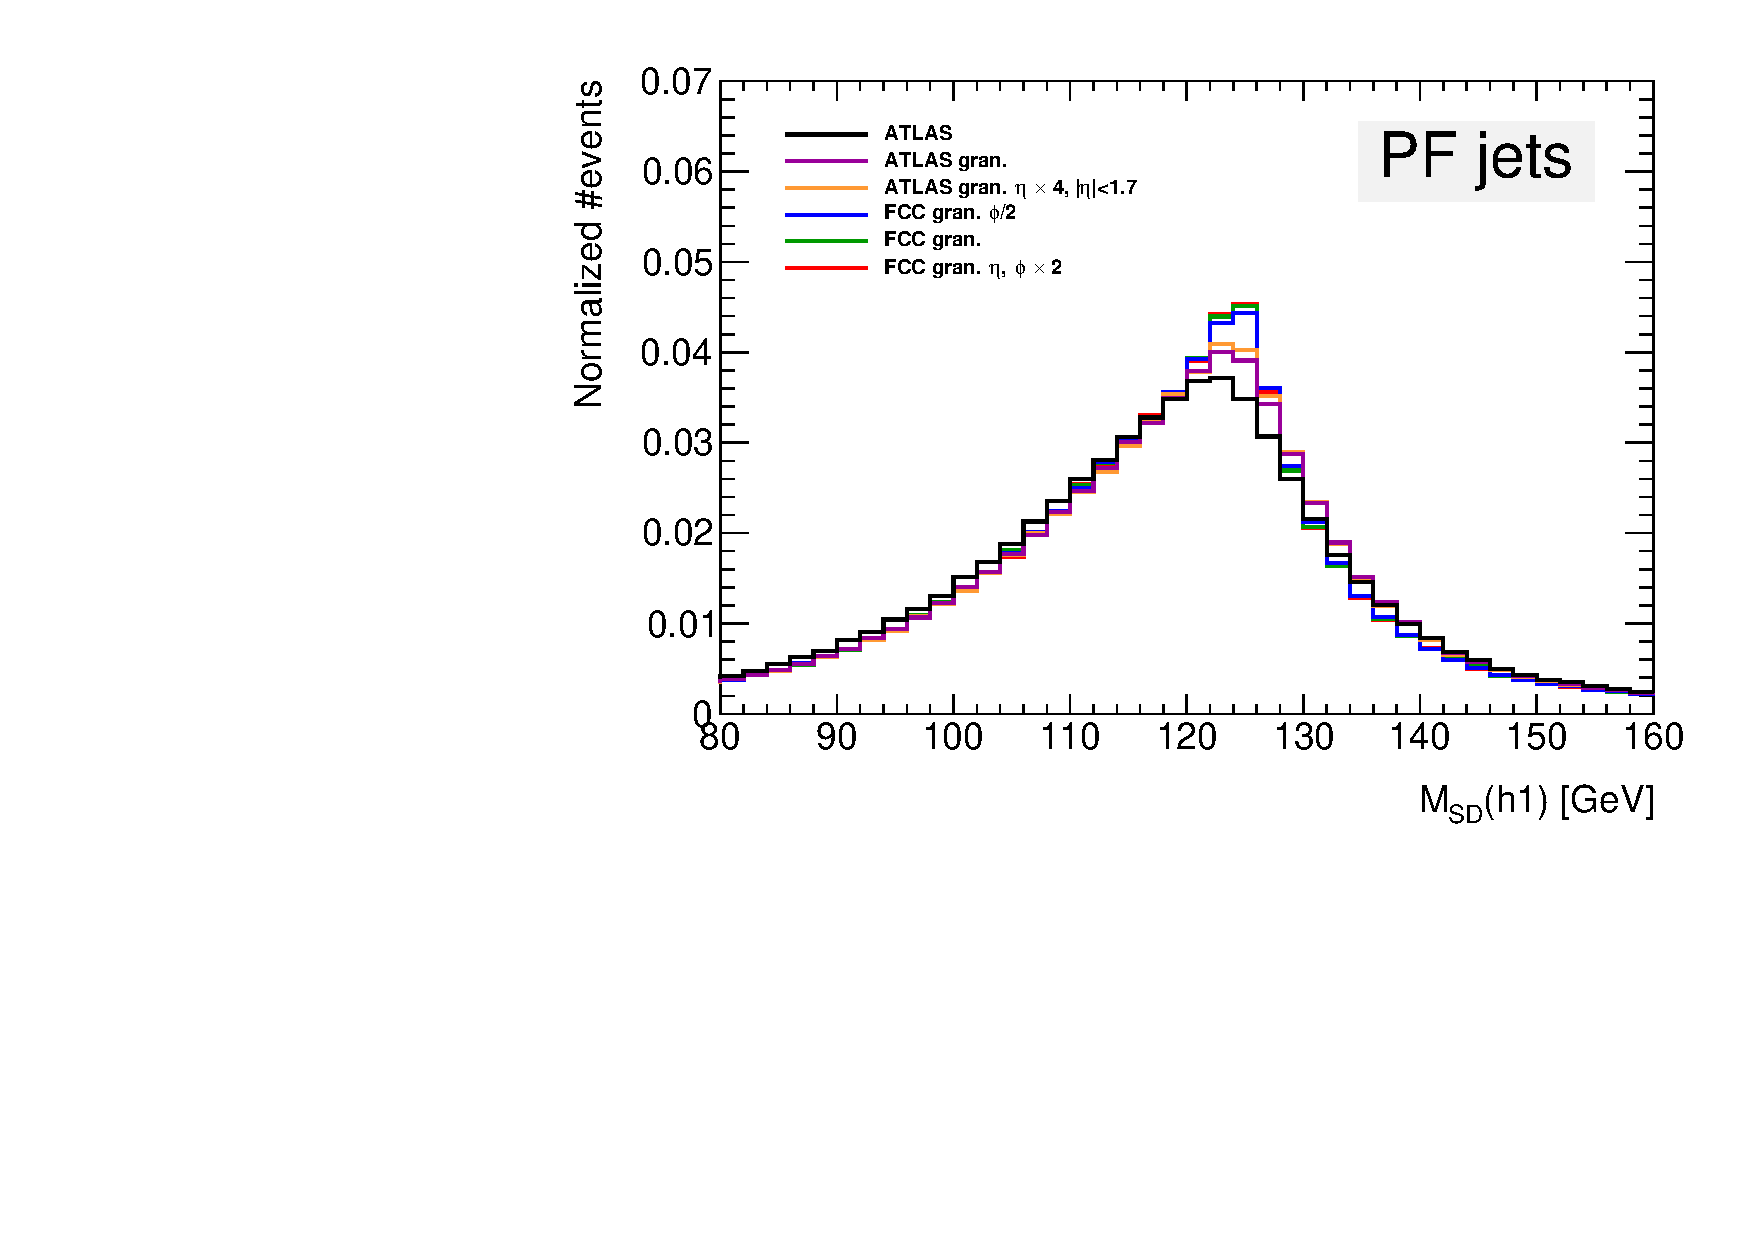
\includegraphics[trim={.55cm 0 0 0},clip,width=\linewidth]{./Figures/M.pdf}
		
		%\caption*{(a)}
	\end{minipage}%
	\begin{minipage}[t]{.5\textwidth}
		\centering
		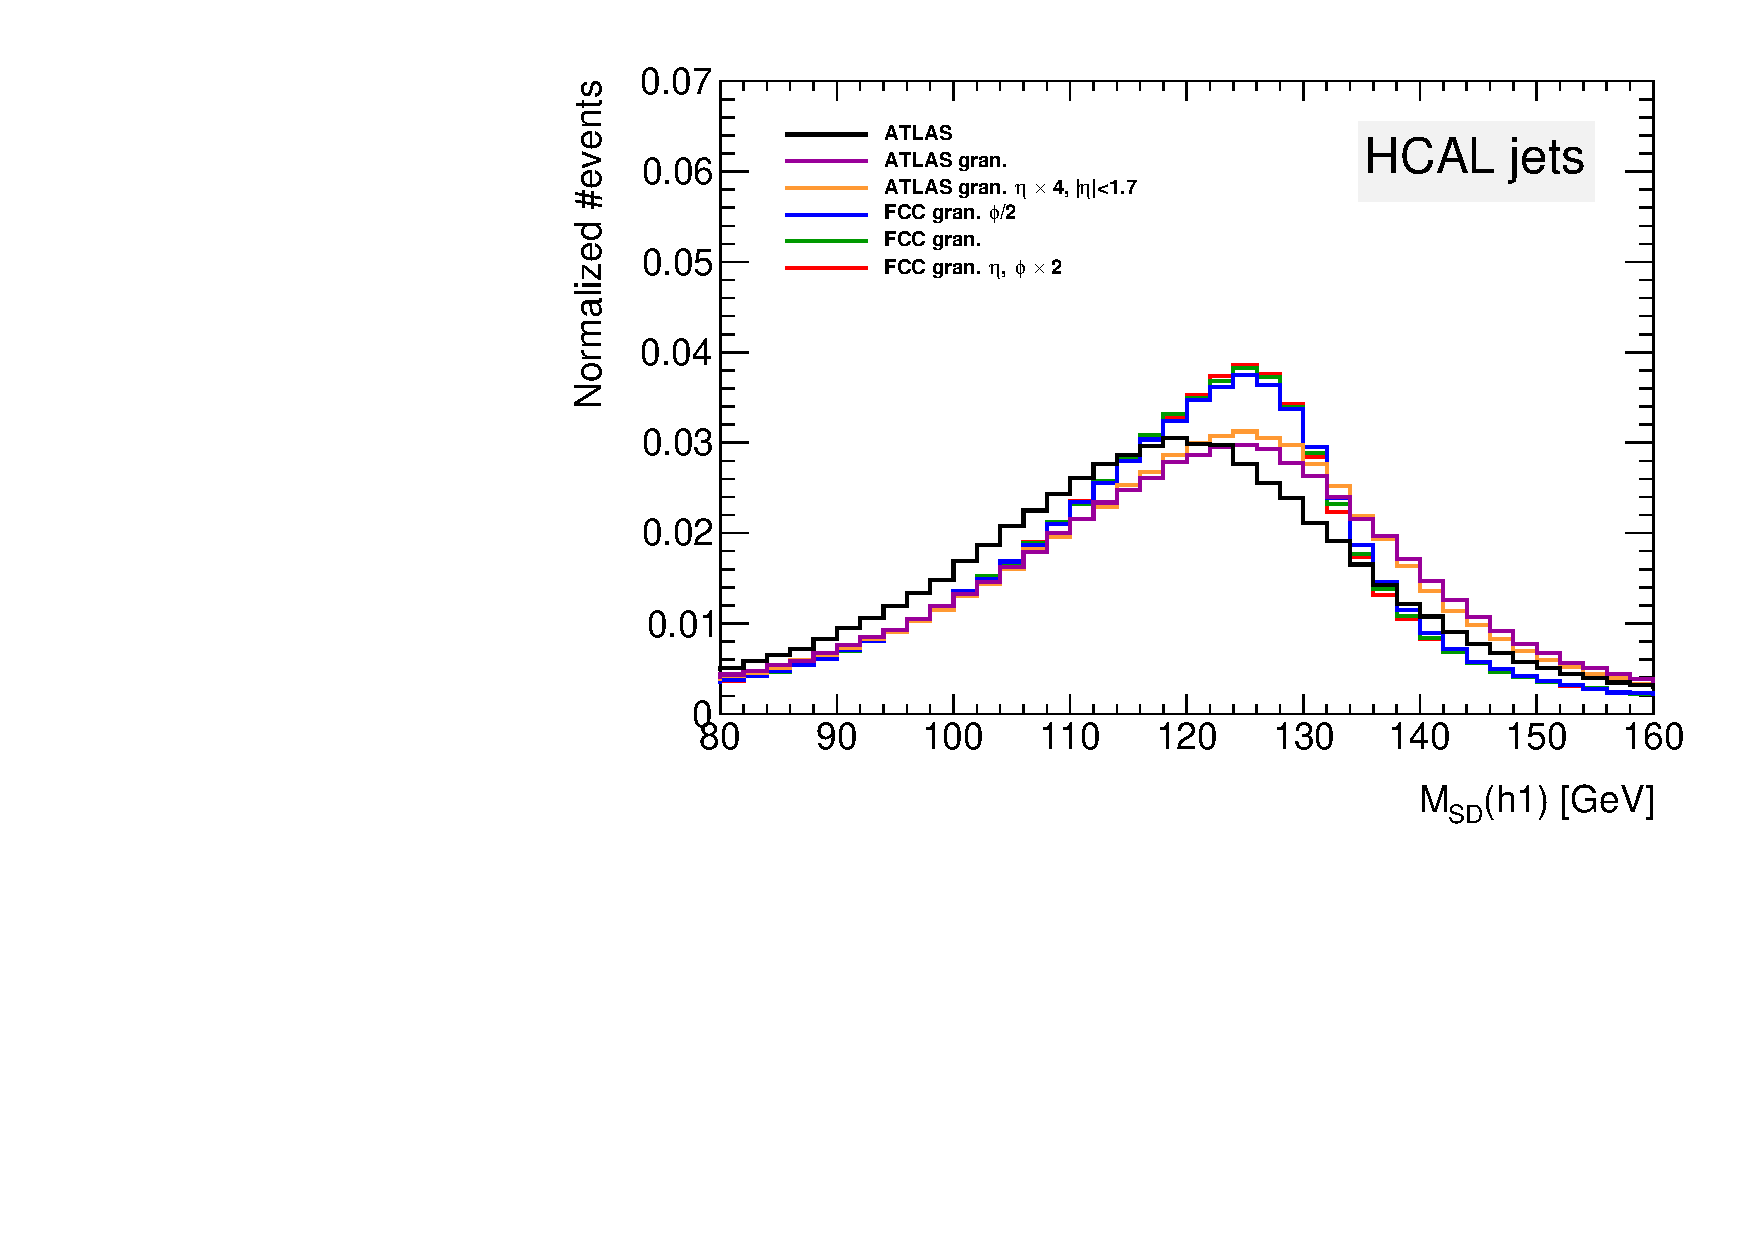
\includegraphics[trim={0 0 .55cm 0},clip,width=\linewidth]{./Figures/MCALO.pdf}
		%\caption*{(b)}
		%\label{fig:CompGran_M_aftercuts}
	\end{minipage}
	
	\begin{minipage}[t]{0.5\textwidth}
		\caption*{(a)}
		\label{fig:CompGran_M}
		%\label{fig1}
	\end{minipage}%%%
	\hfill
	\begin{minipage}[t]{0.5\textwidth}
		\caption*{(b)}
		%\label{fig2}
	\end{minipage}
	\caption{Leading Higgs candidate softdrop mass after the pre-selection cuts for particle flow (a) and calorimeter (b) jets. The colors indicate the different detector configurations. The x axis range is from $80$ GeV to $160$ GeV in order to make the differences between the histograms more clear.}
	\label{fig:CompGran}
\end{figure}

\begin{figure}
	\centering
	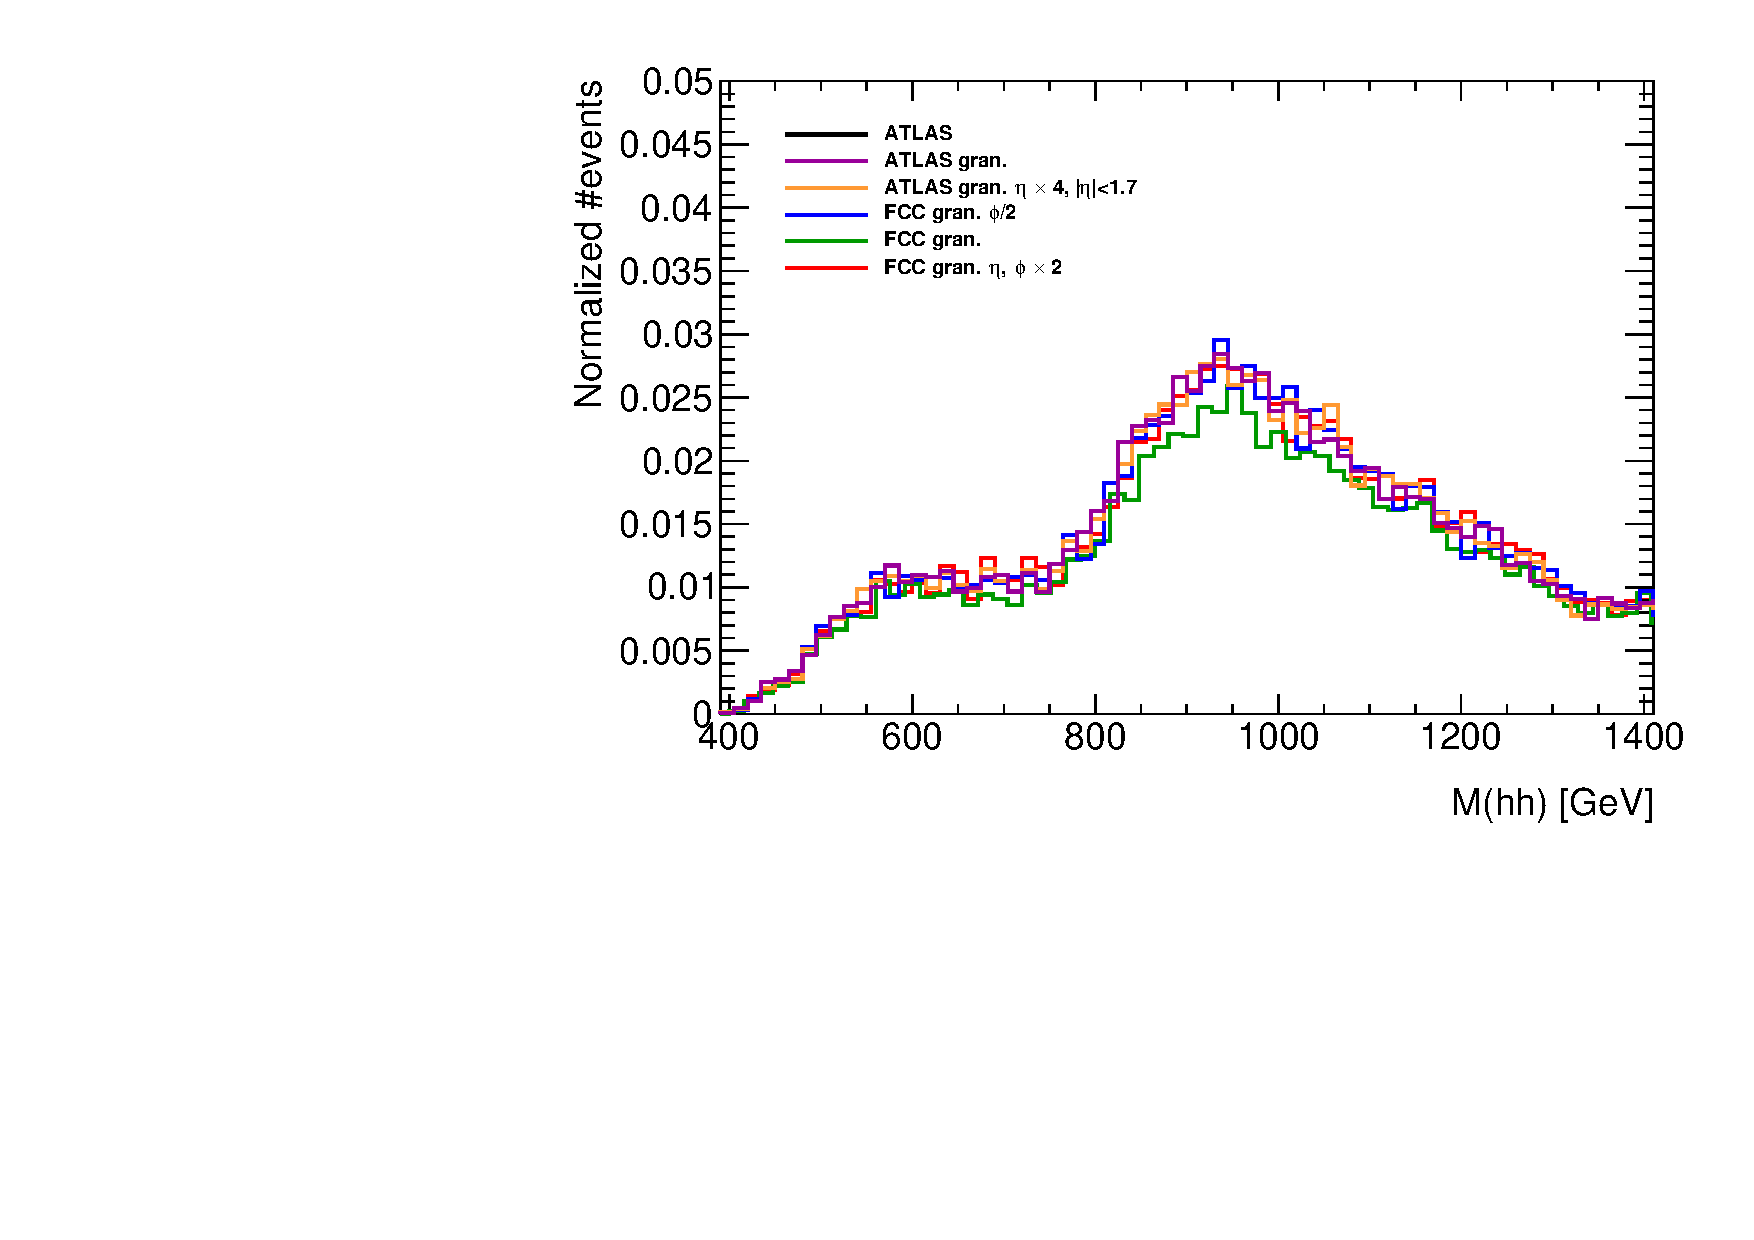
\includegraphics[width=0.5\linewidth]{./Figures/Mhh_after.pdf}
	\caption{Invariant mass of the Higgs pair for the SM signal. The plots include the events that pass all the analysis cuts. The colors indicate the different detector configurations.}
	\label{fig:CompGran_Mhh}
\end{figure}

\begin{figure}
	\centering
	\begin{minipage}[t]{.5\textwidth}
		\centering
		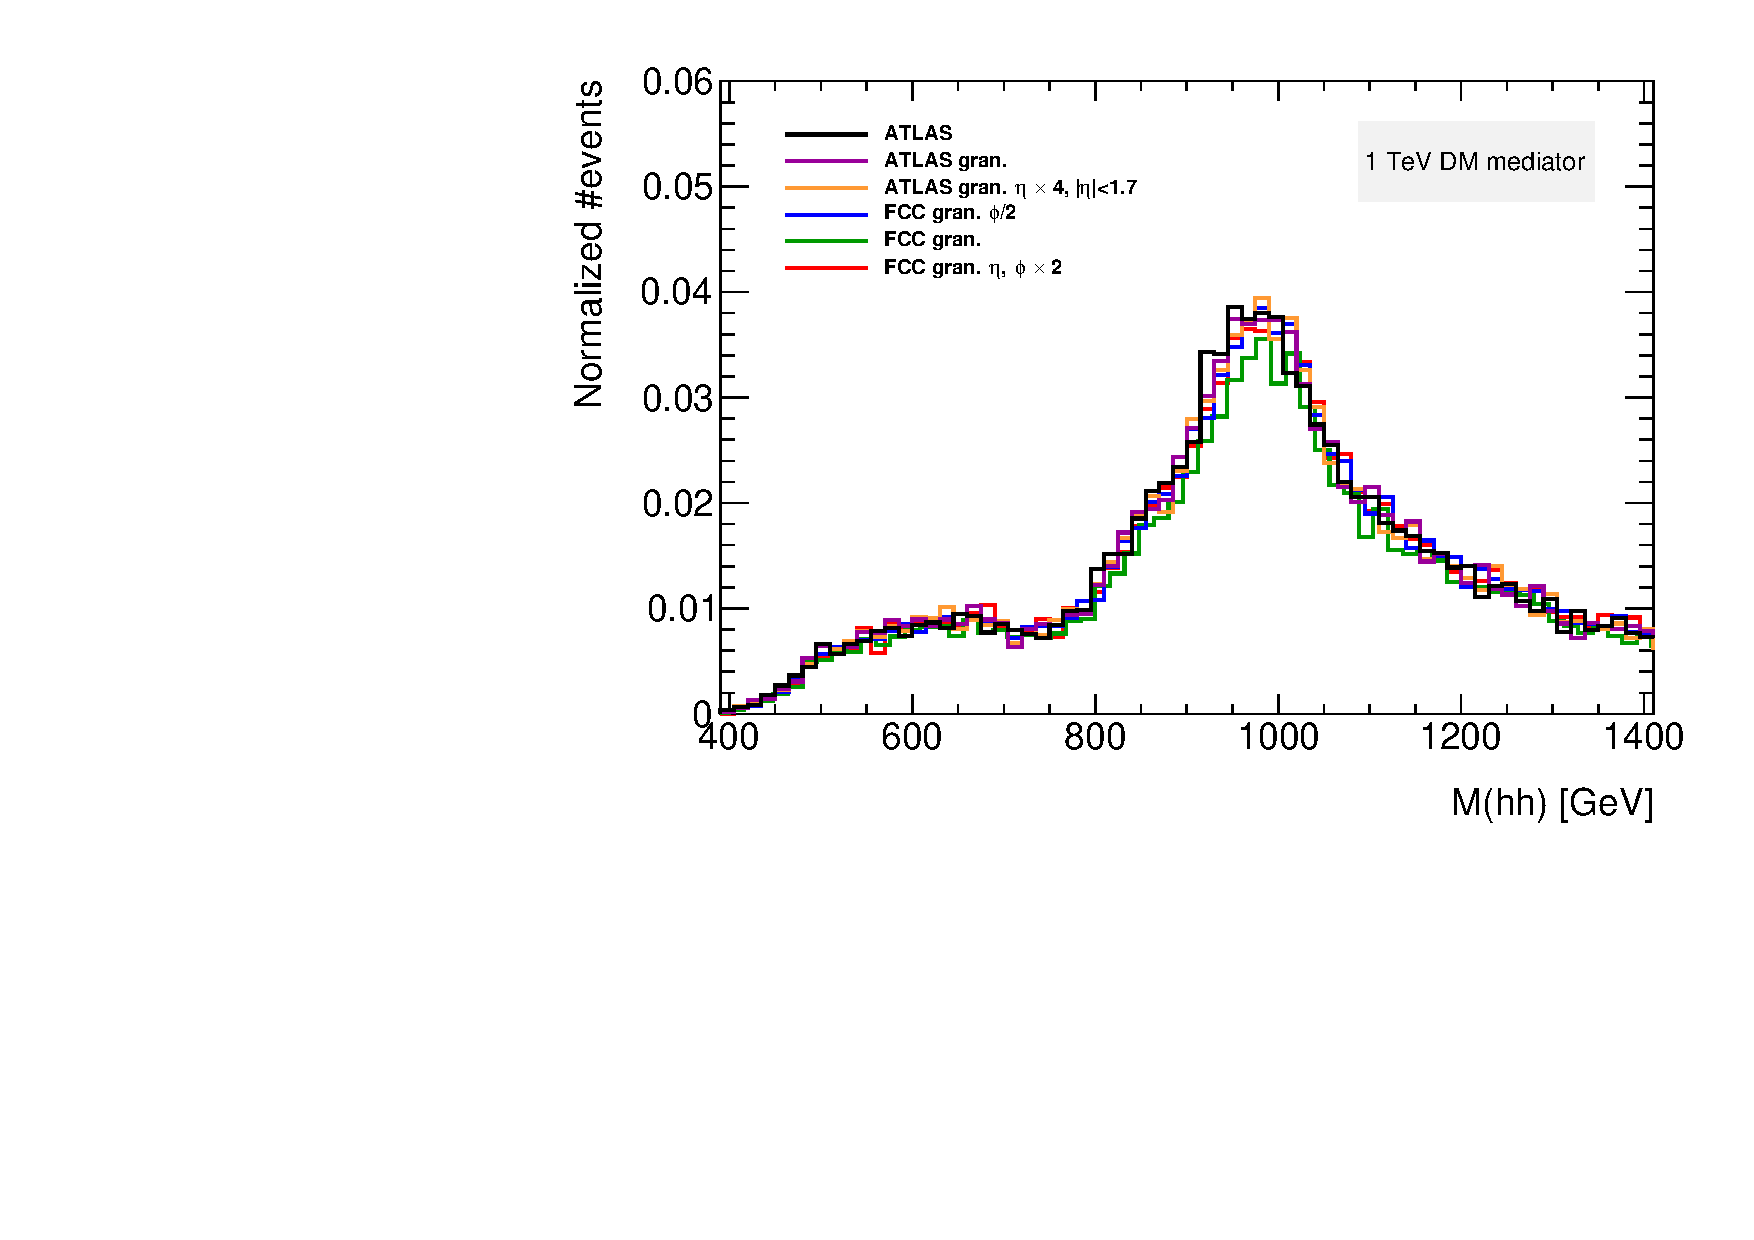
\includegraphics[trim={.55cm 0 0 0},clip,width=\linewidth]{./Figures/MhhX_after.pdf}
		%\label{fig:CompGran_M}
		%\caption*{(a)}
	\end{minipage}%
	\begin{minipage}[t]{.5\textwidth}
		\centering
		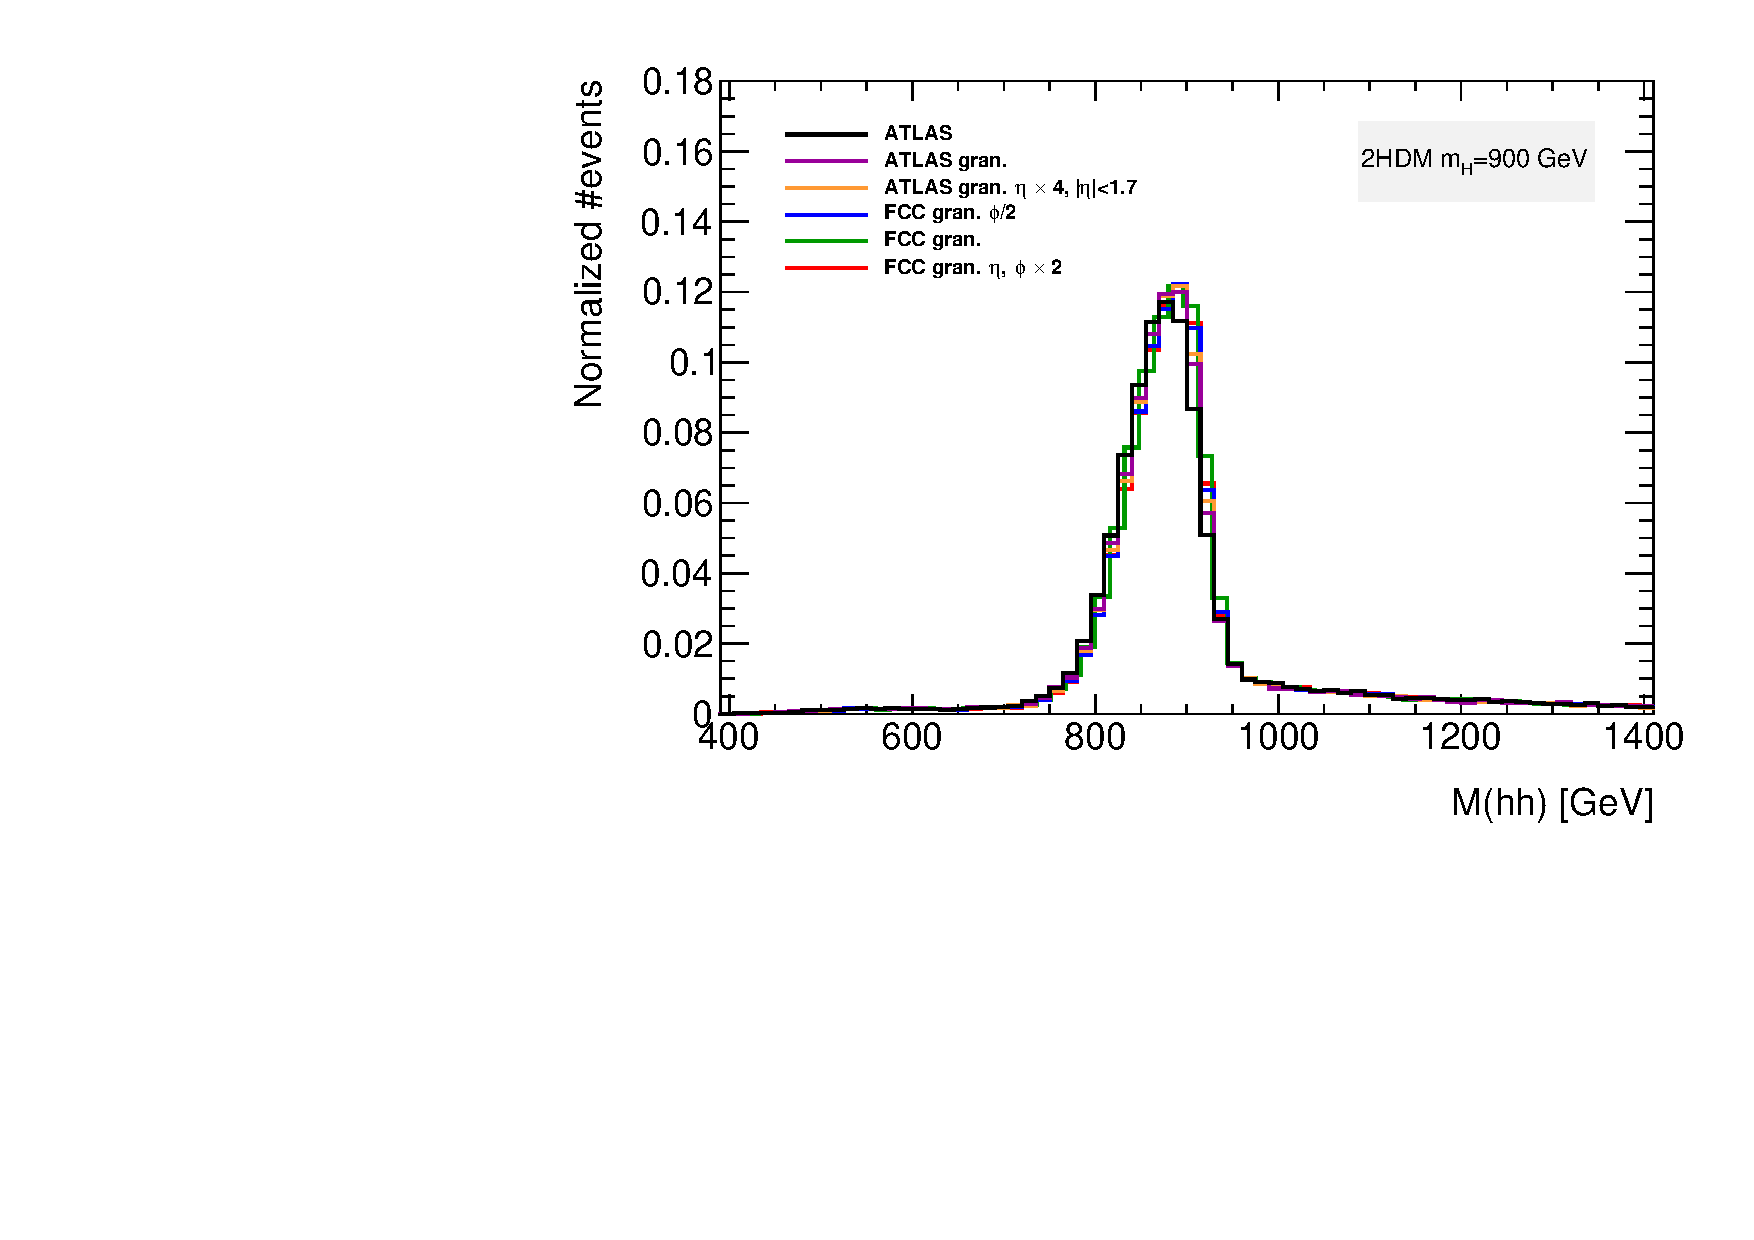
\includegraphics[trim={0 0 .55cm 0},clip,width=\linewidth]{./Figures/Mhh2HDM_after.pdf}
		%\caption*{(b)}
		%\label{fig:CompGran_M_aftercuts}
	\end{minipage}
	
	\begin{minipage}[t]{0.5\textwidth}
		\caption*{(a)}
		%\label{fig1}
	\end{minipage}%%%
	\hfill
	\begin{minipage}[t]{0.5\textwidth}
		\caption*{(b)}
		%\label{fig2}
	\end{minipage}
	
	\caption{(a) Invariant mass of the Higgs pair for the $1$ TeV DM mediator, (b) Invariant mass of the Higgs pair for the 2HDM with $m_H=900$ GeV. The plots include the events that pass all the analysis cuts. The colors indicate the different detector configurations.}
	\label{fig:CompGran1}
\end{figure}

\begin{figure}
	\centering
	\begin{minipage}[t]{.5\textwidth}
		\centering
		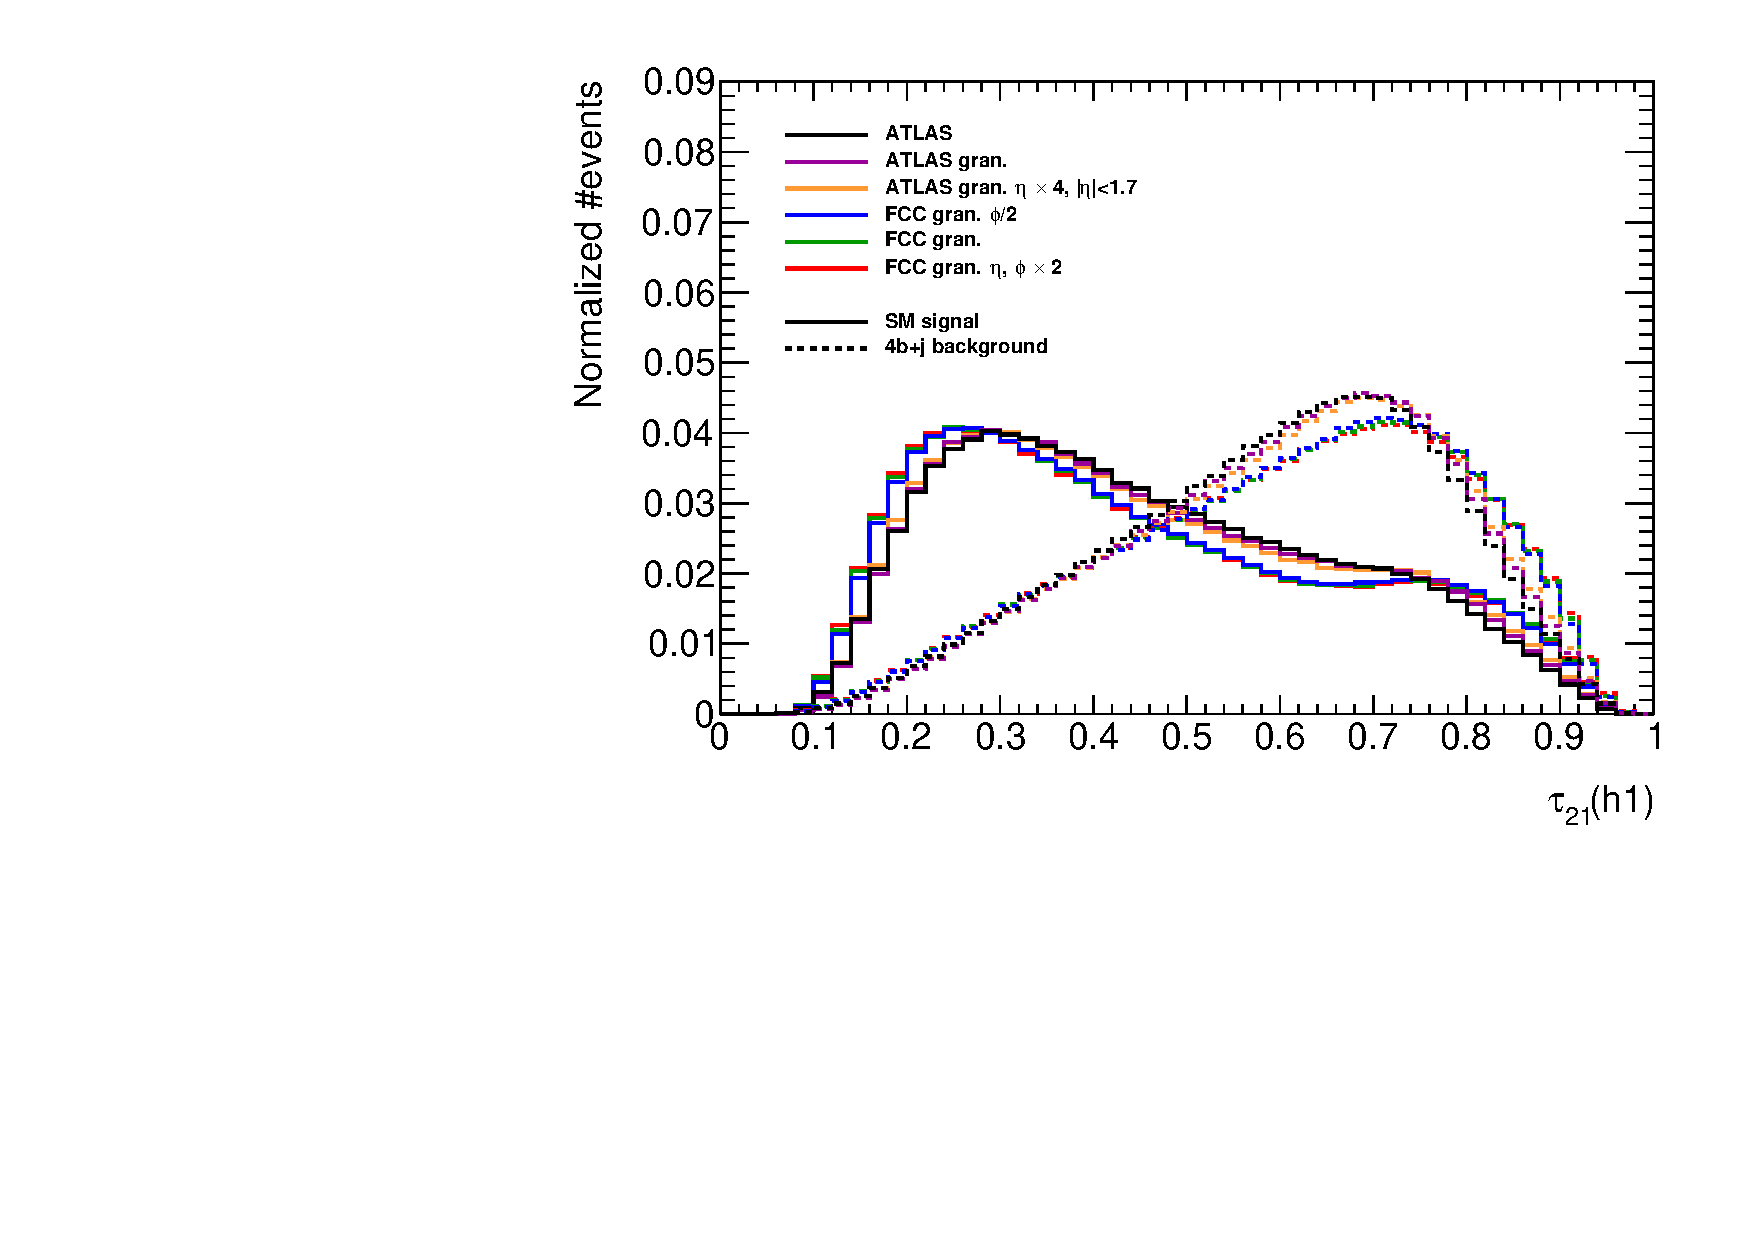
\includegraphics[trim={.65cm 0 0 0},clip,width=\linewidth]{./Figures/tau21.pdf}
	\end{minipage}%
	\begin{minipage}[t]{.5\textwidth}
		\centering
		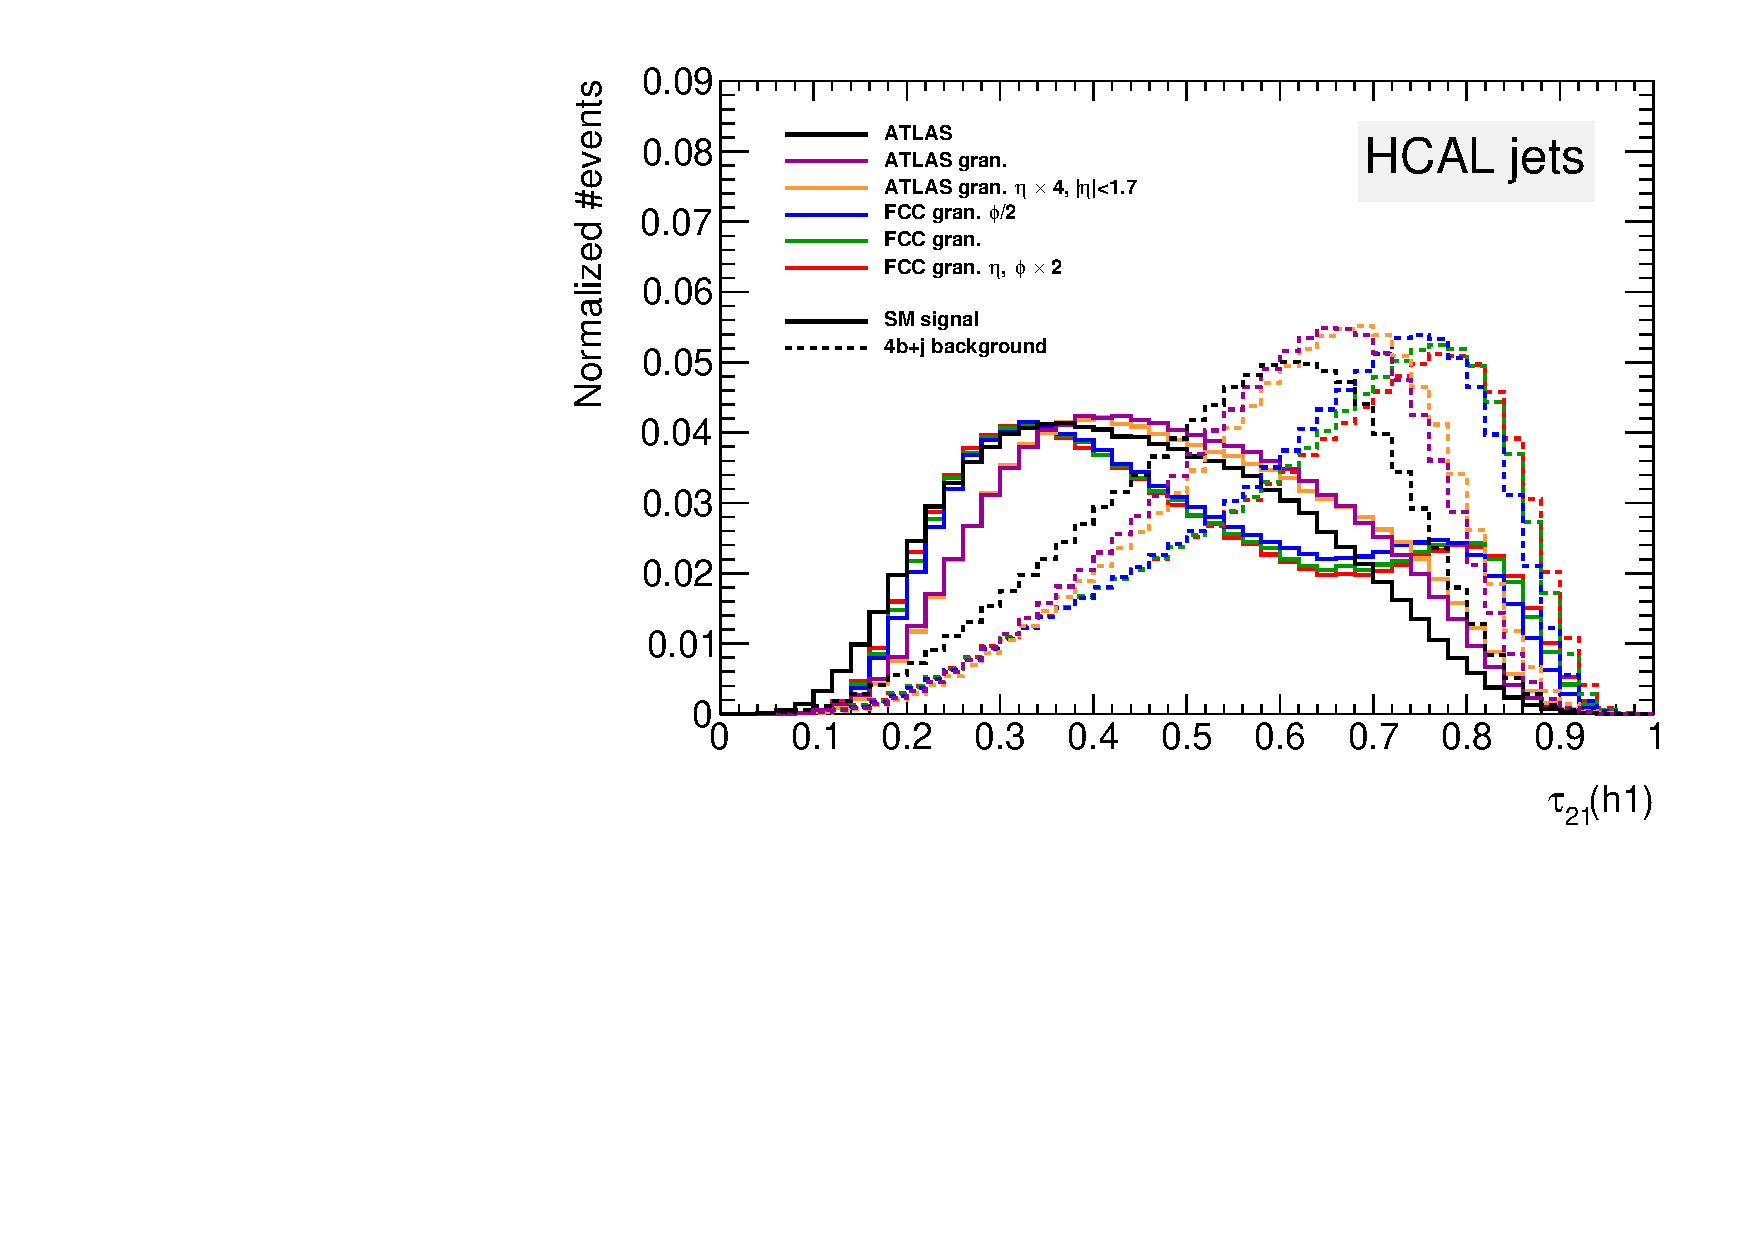
\includegraphics[trim={0 0 .65cm 0},clip,width=\linewidth]{./Figures/tau21CALO.pdf}
	\end{minipage}
	
	\begin{minipage}[t]{0.5\textwidth}
		\caption*{(a)}
		%\label{fig1}
	\end{minipage}%%%
	\hfill
	\begin{minipage}[t]{0.5\textwidth}
		\caption*{(b)}
		%\label{fig2}
	\end{minipage}
	\caption{(a) Leading Higgs candidate $\tau_{21}$ distribution for eflow jets, (b) Leading Higgs candidate $\tau_{21}$ distribution for HCAL jets. The colors indicate the different detector configurations. The distributions are shown for the signal (filled lines) and for the $4b+j$ background (dashed lines).}
	\label{fig:CompGran_sub}
\end{figure}

%\begin{figure}
%	\centering
%	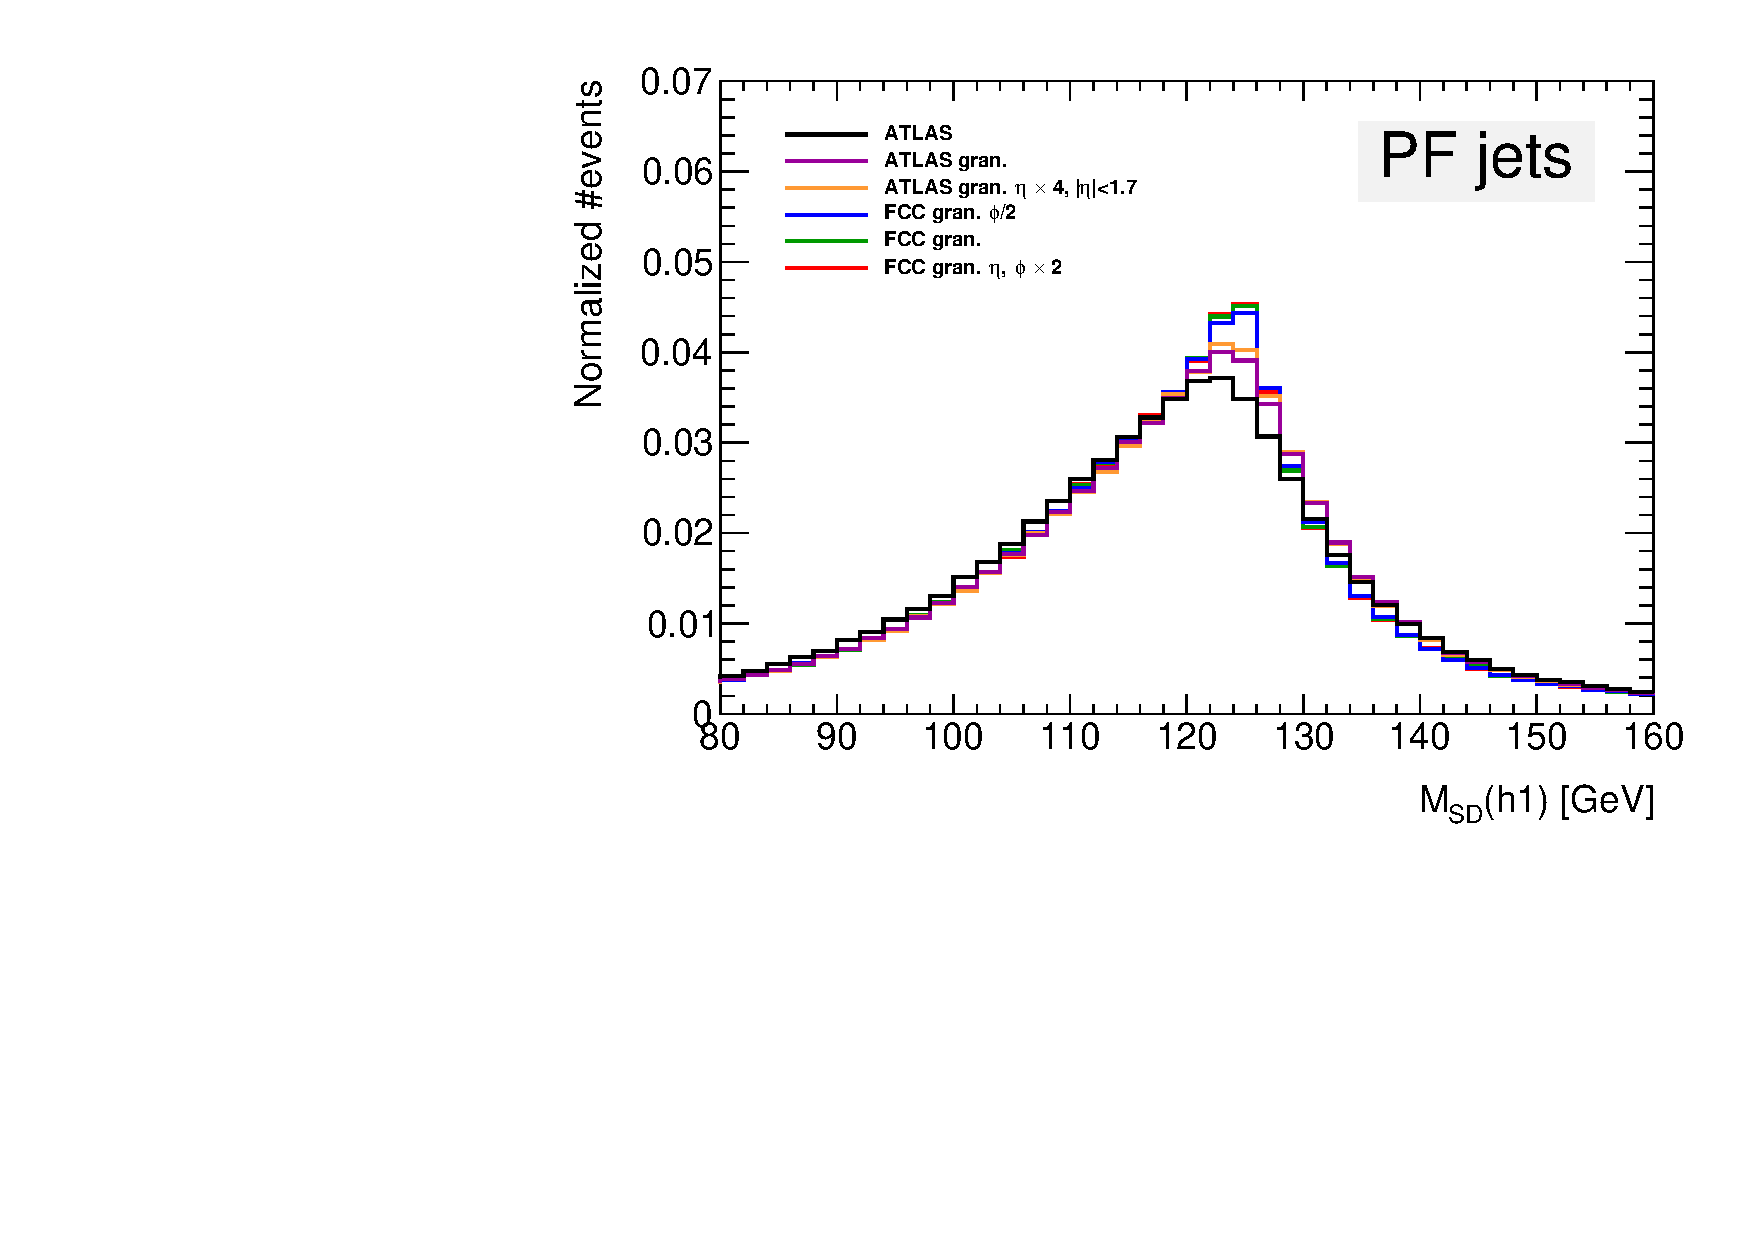
\includegraphics[width=\linewidth]{./Figures/M.pdf}
%	\label{fig:CompGran_M}
%	\caption{Leading Higgs candidate softdrop mass plot for the different detector configurations for the SM signal sample. This plot contains all the signal events that passed all the cuts of the baseline analysis. Note that the x axis range is from $80$ GeV to $160$ GeV in order to make the differences between the histograms more clear.}
%\end{figure}
%
%\begin{figure}
%	\centering
%	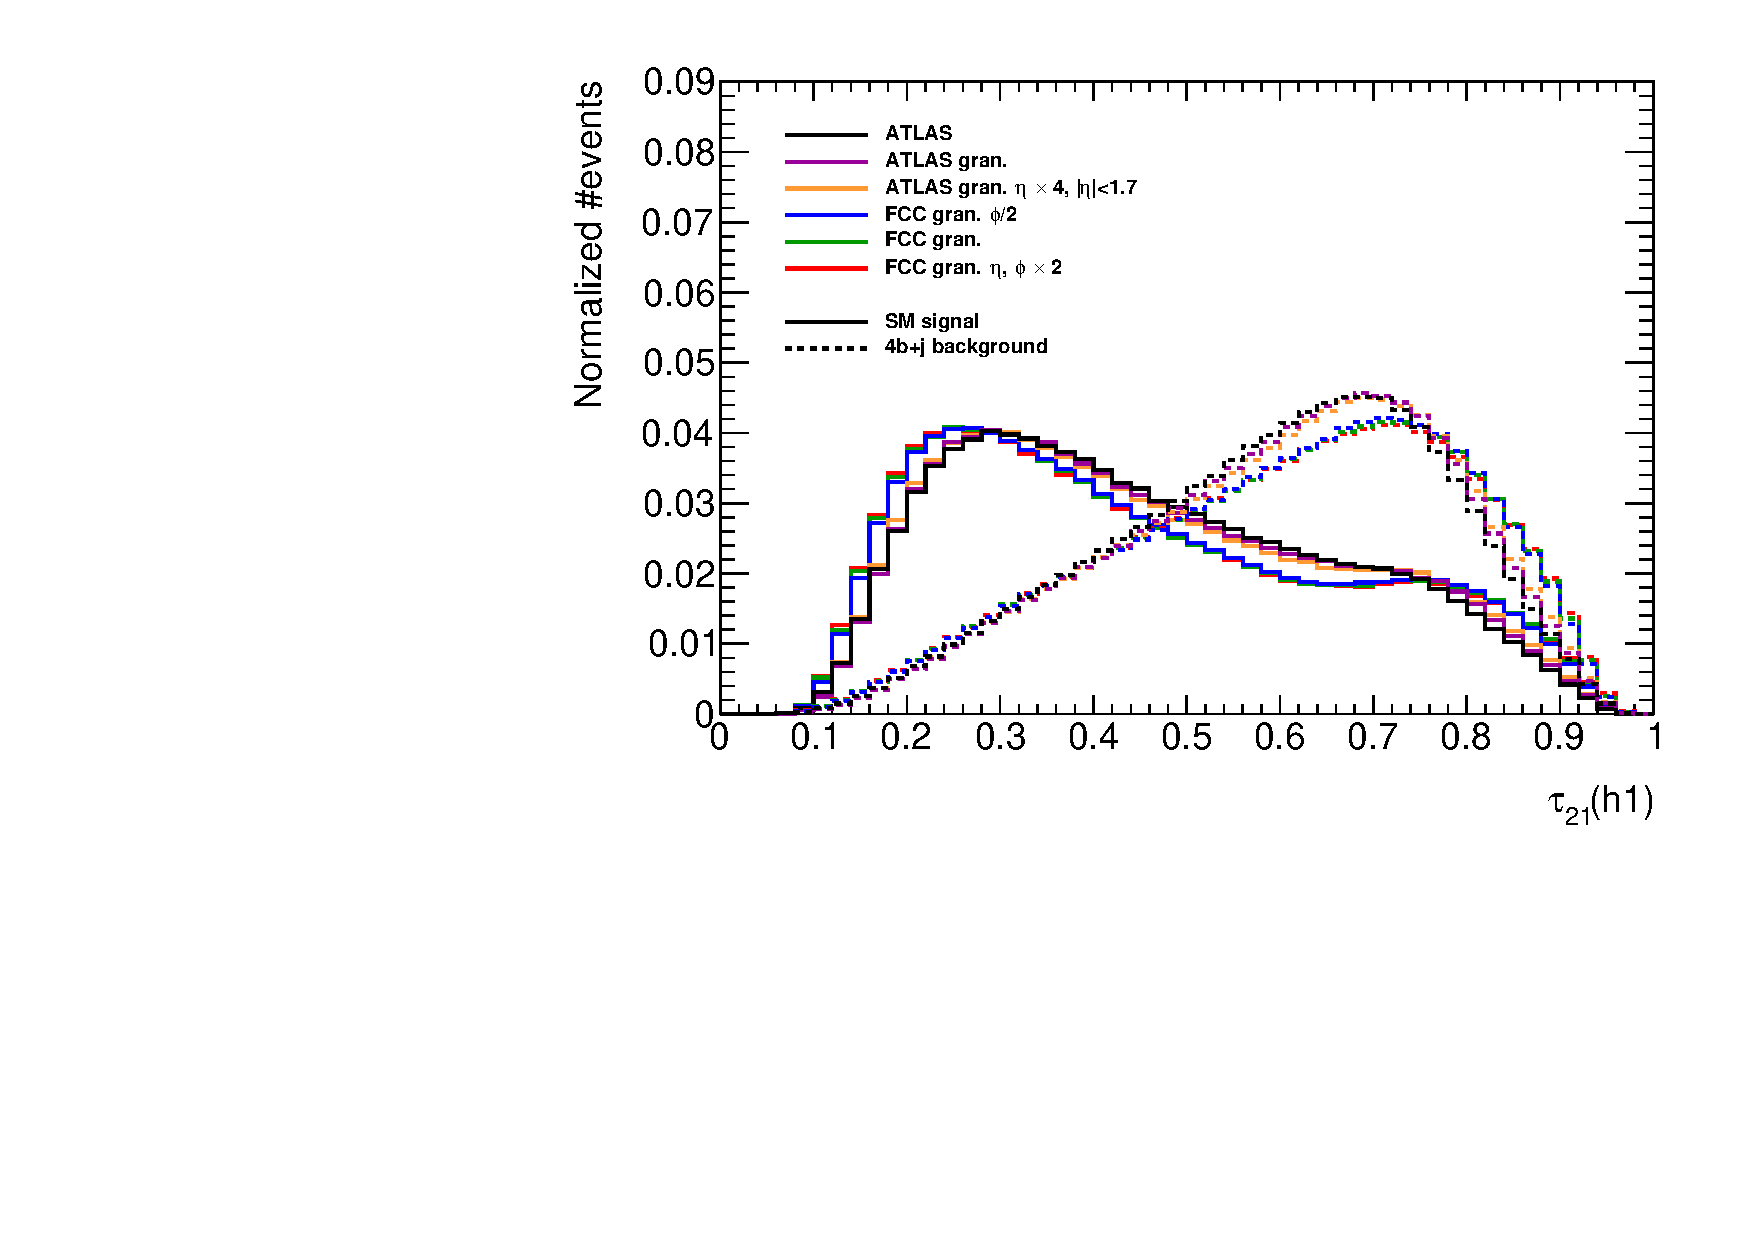
\includegraphics[width=\linewidth]{./Figures/tau21.pdf}
%	\label{fig:CompGran_tau21}
%	\caption{Leading Higgs candidate $\tau_{21}$ plot for the different detector configurations for the SM signal sample. This plot contains all the signal events that passed all the cuts of the baseline analysis.}
%\end{figure}

\begin{figure}
	\centering
	\begin{minipage}{.5\textwidth}
		\centering
		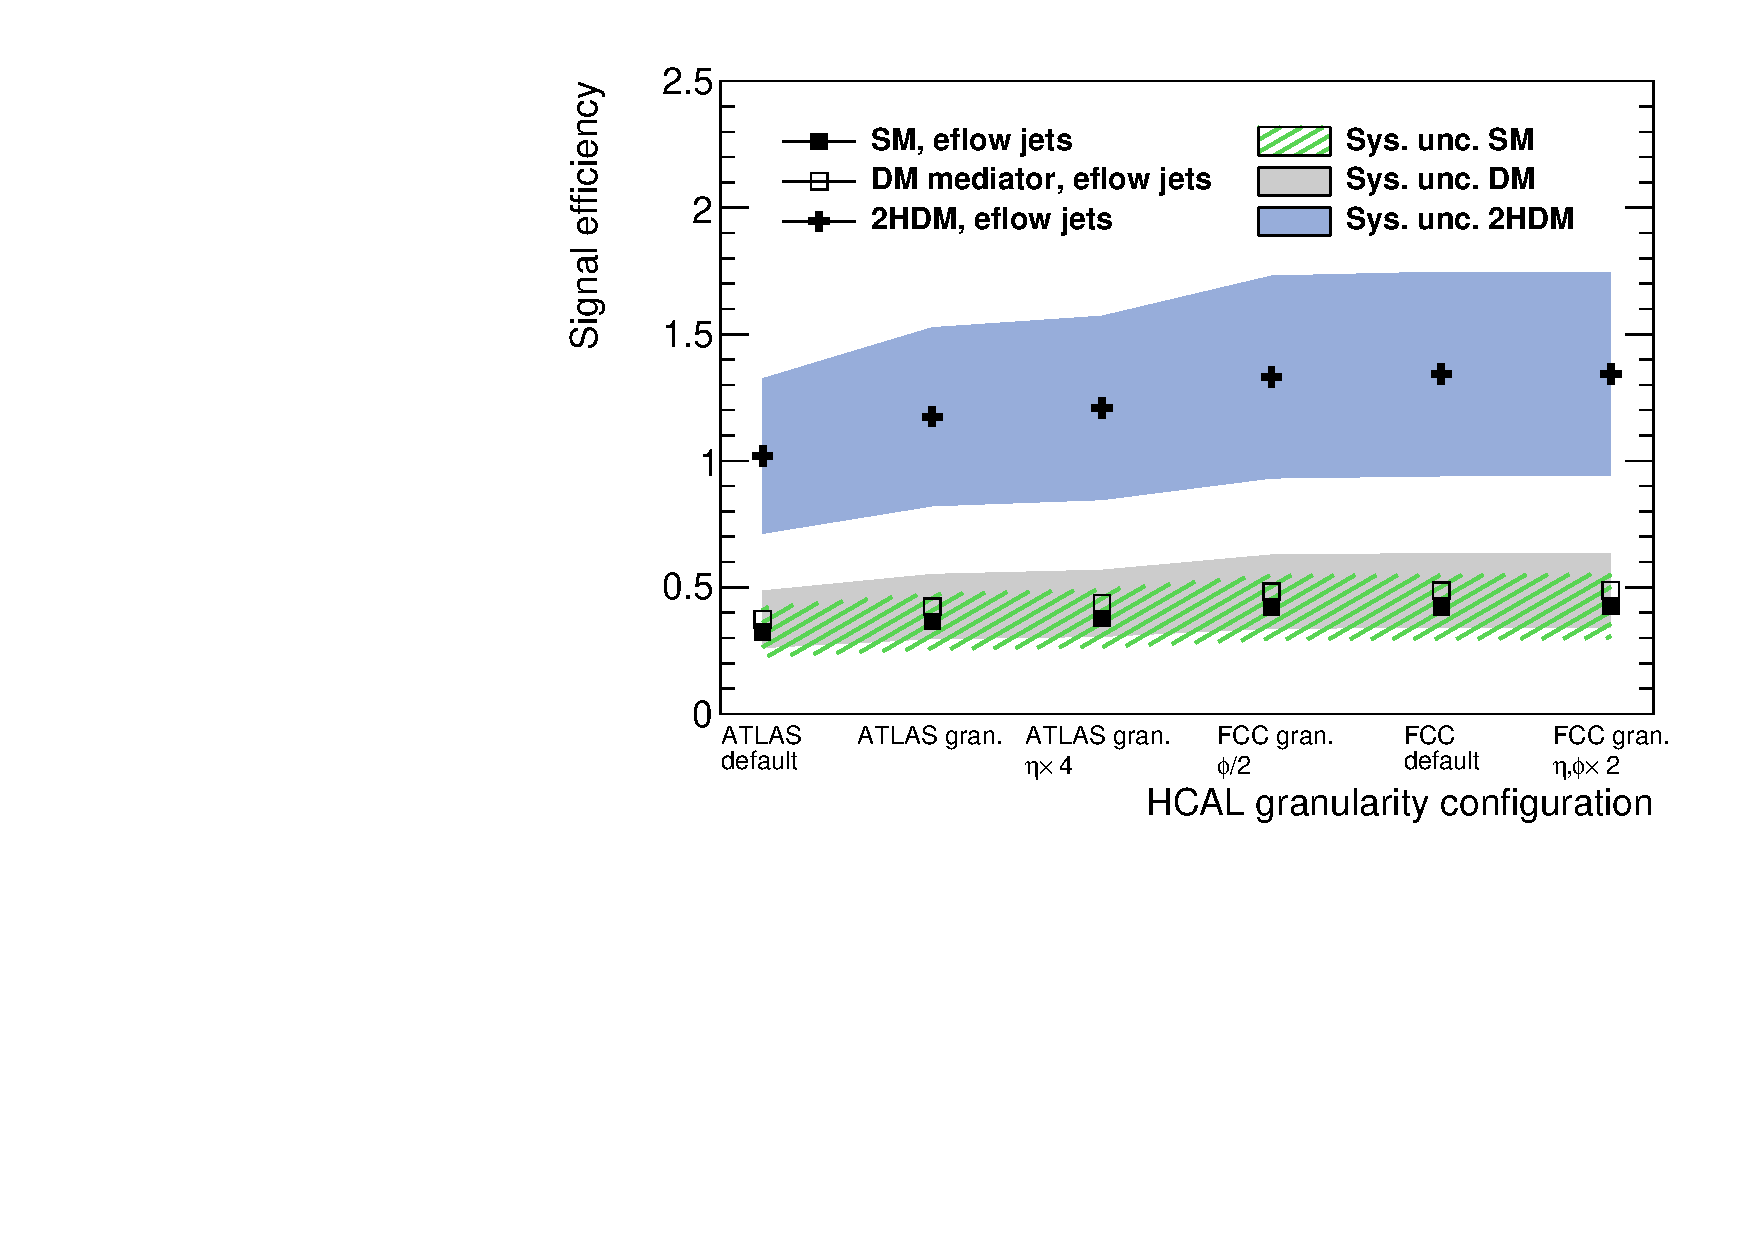
\includegraphics[trim={.6cm 0 0 0},clip,width=\linewidth]{./Figures/EffvsGran_PFjets.pdf}
	\end{minipage}%
	\begin{minipage}{.5\textwidth}
		\centering
		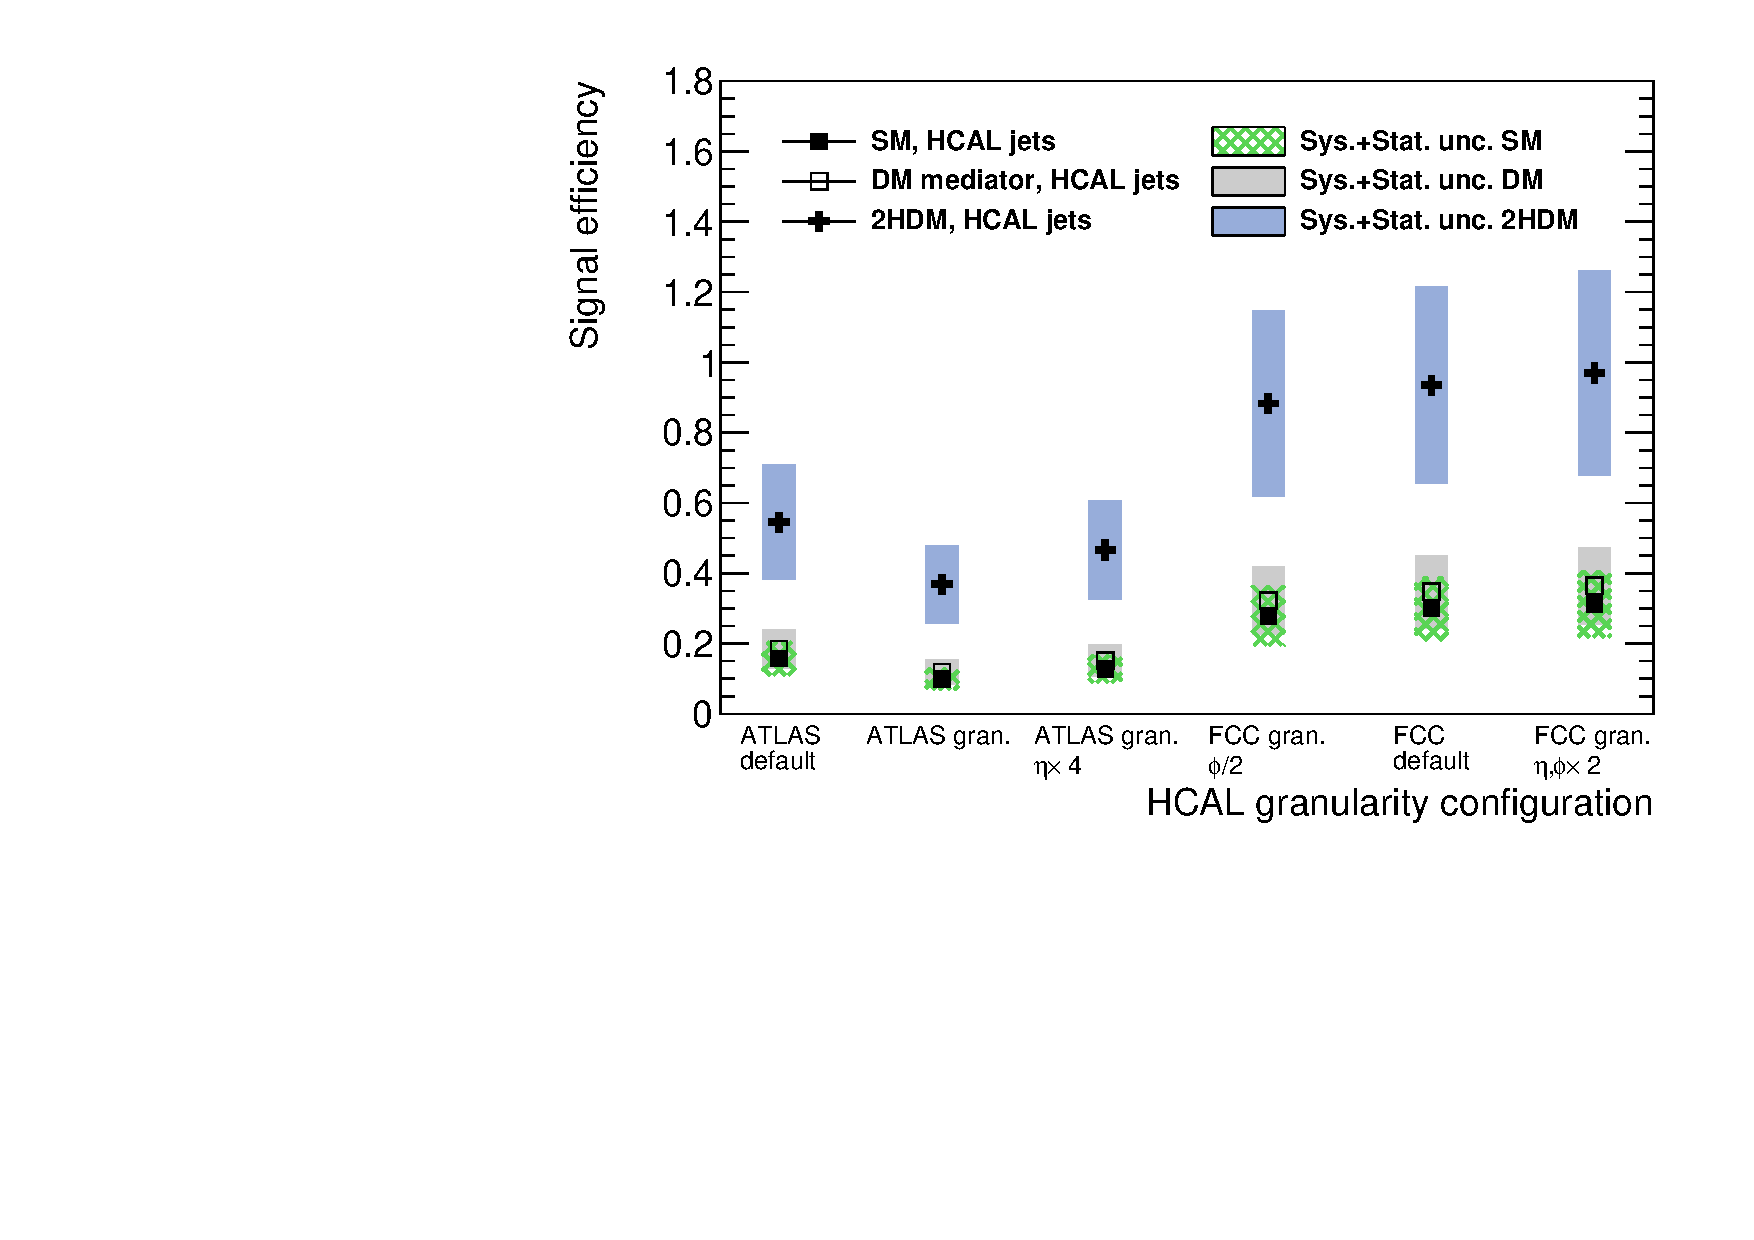
\includegraphics[trim={0 0 .6cm 0},clip,width=\linewidth]{./Figures/EffvsGran_CALOjets.pdf}
	\end{minipage}
	\begin{minipage}[t]{0.5\textwidth}
		\caption*{(a)}
		%\label{fig1}
	\end{minipage}%%%
	\hfill
	\begin{minipage}[t]{0.5\textwidth}
		\caption*{(b)}
		%\label{fig2}
	\end{minipage}
	\caption{Signal efficiency as a function of the detector configuration for particle flow jets (a) and for calorimeter jets (b). Three signal models are shown: SM (filled squares), $1$ TeV DM mediator (empty squares) and type II 2HDM with $m_H=900$ GeV (crosses). The error bars are drawn but are smaller than the markers.}
	\label{fig:EffvsGran}
\end{figure}

\begin{figure}
	\centering
	\begin{minipage}{.5\textwidth}
		\centering
		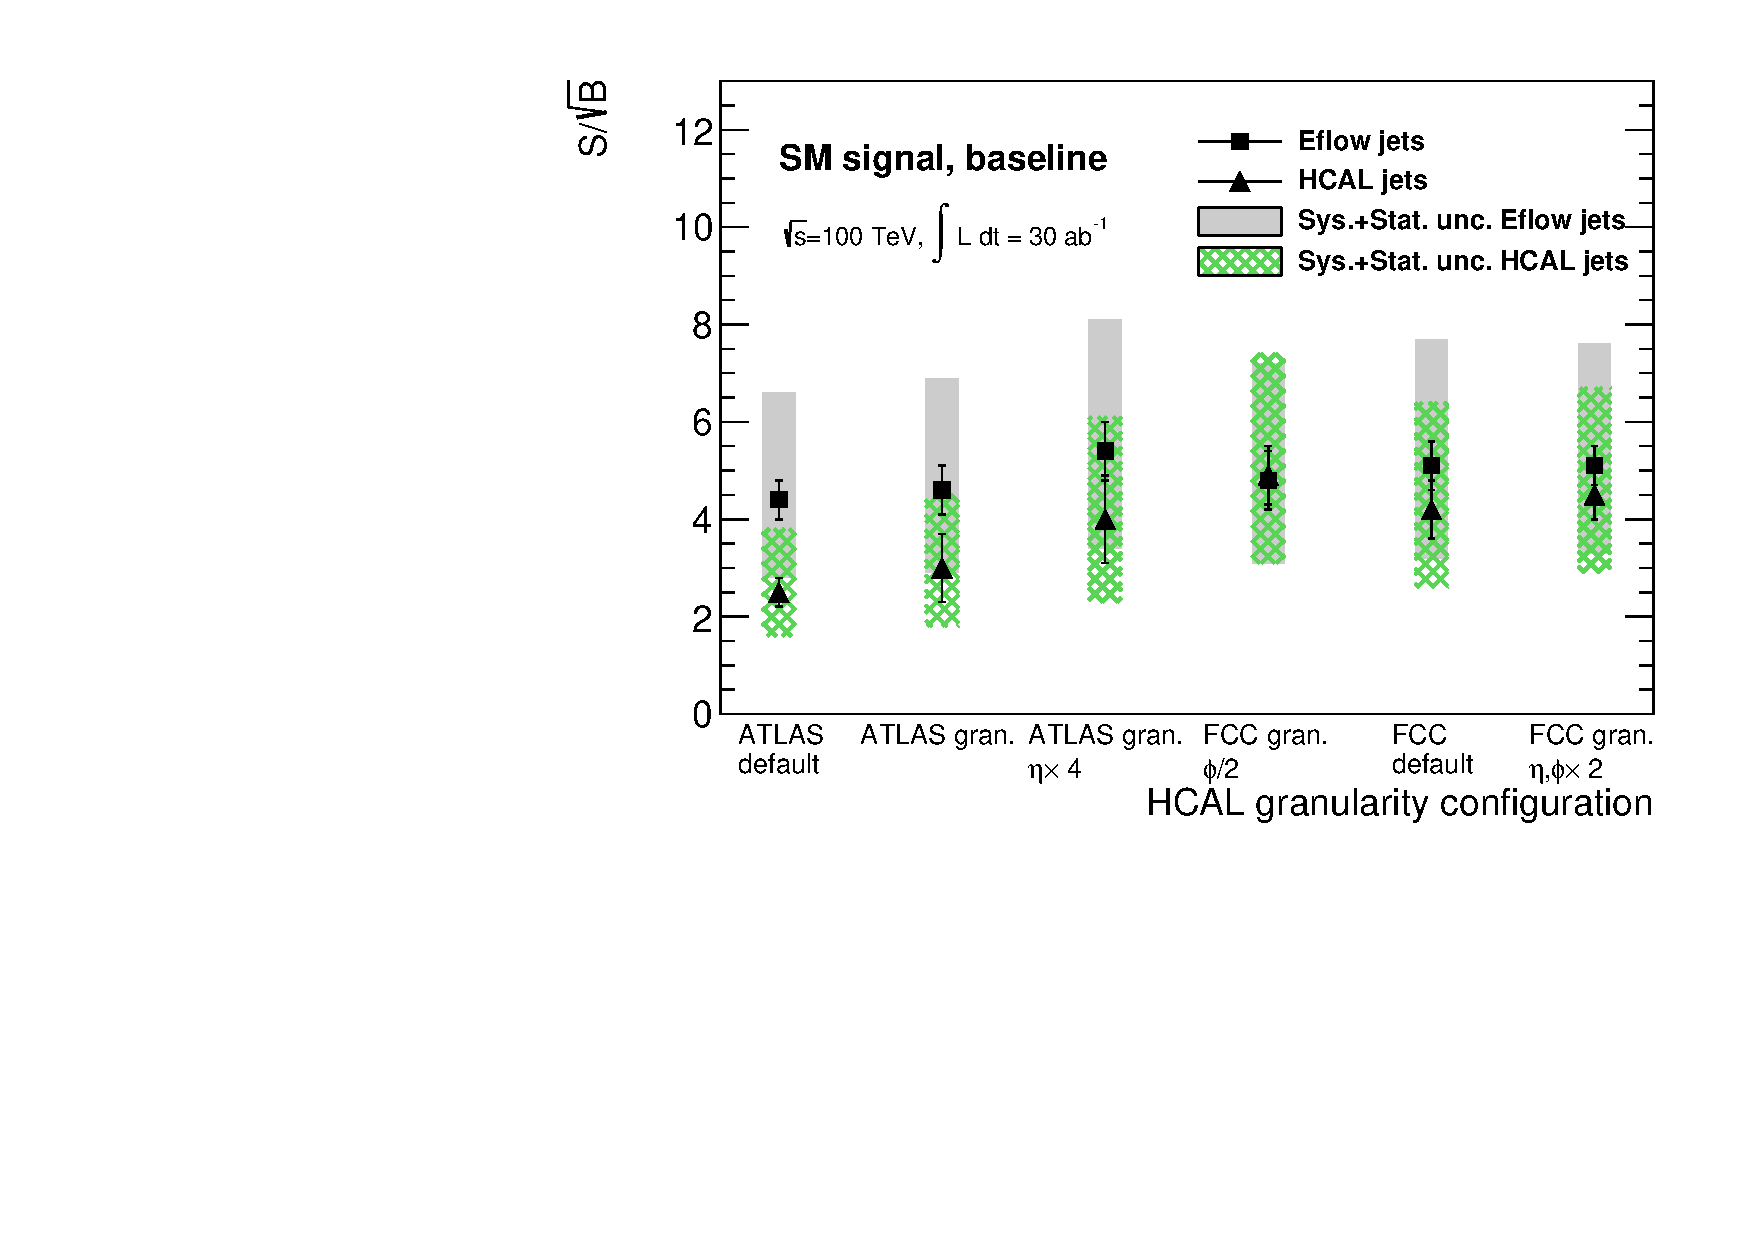
\includegraphics[trim={.6cm 0 0 0},clip,width=\linewidth]{./Figures/SSBvsGran_SM.pdf}
	\end{minipage}%
	\begin{minipage}{.5\textwidth}
		\centering
		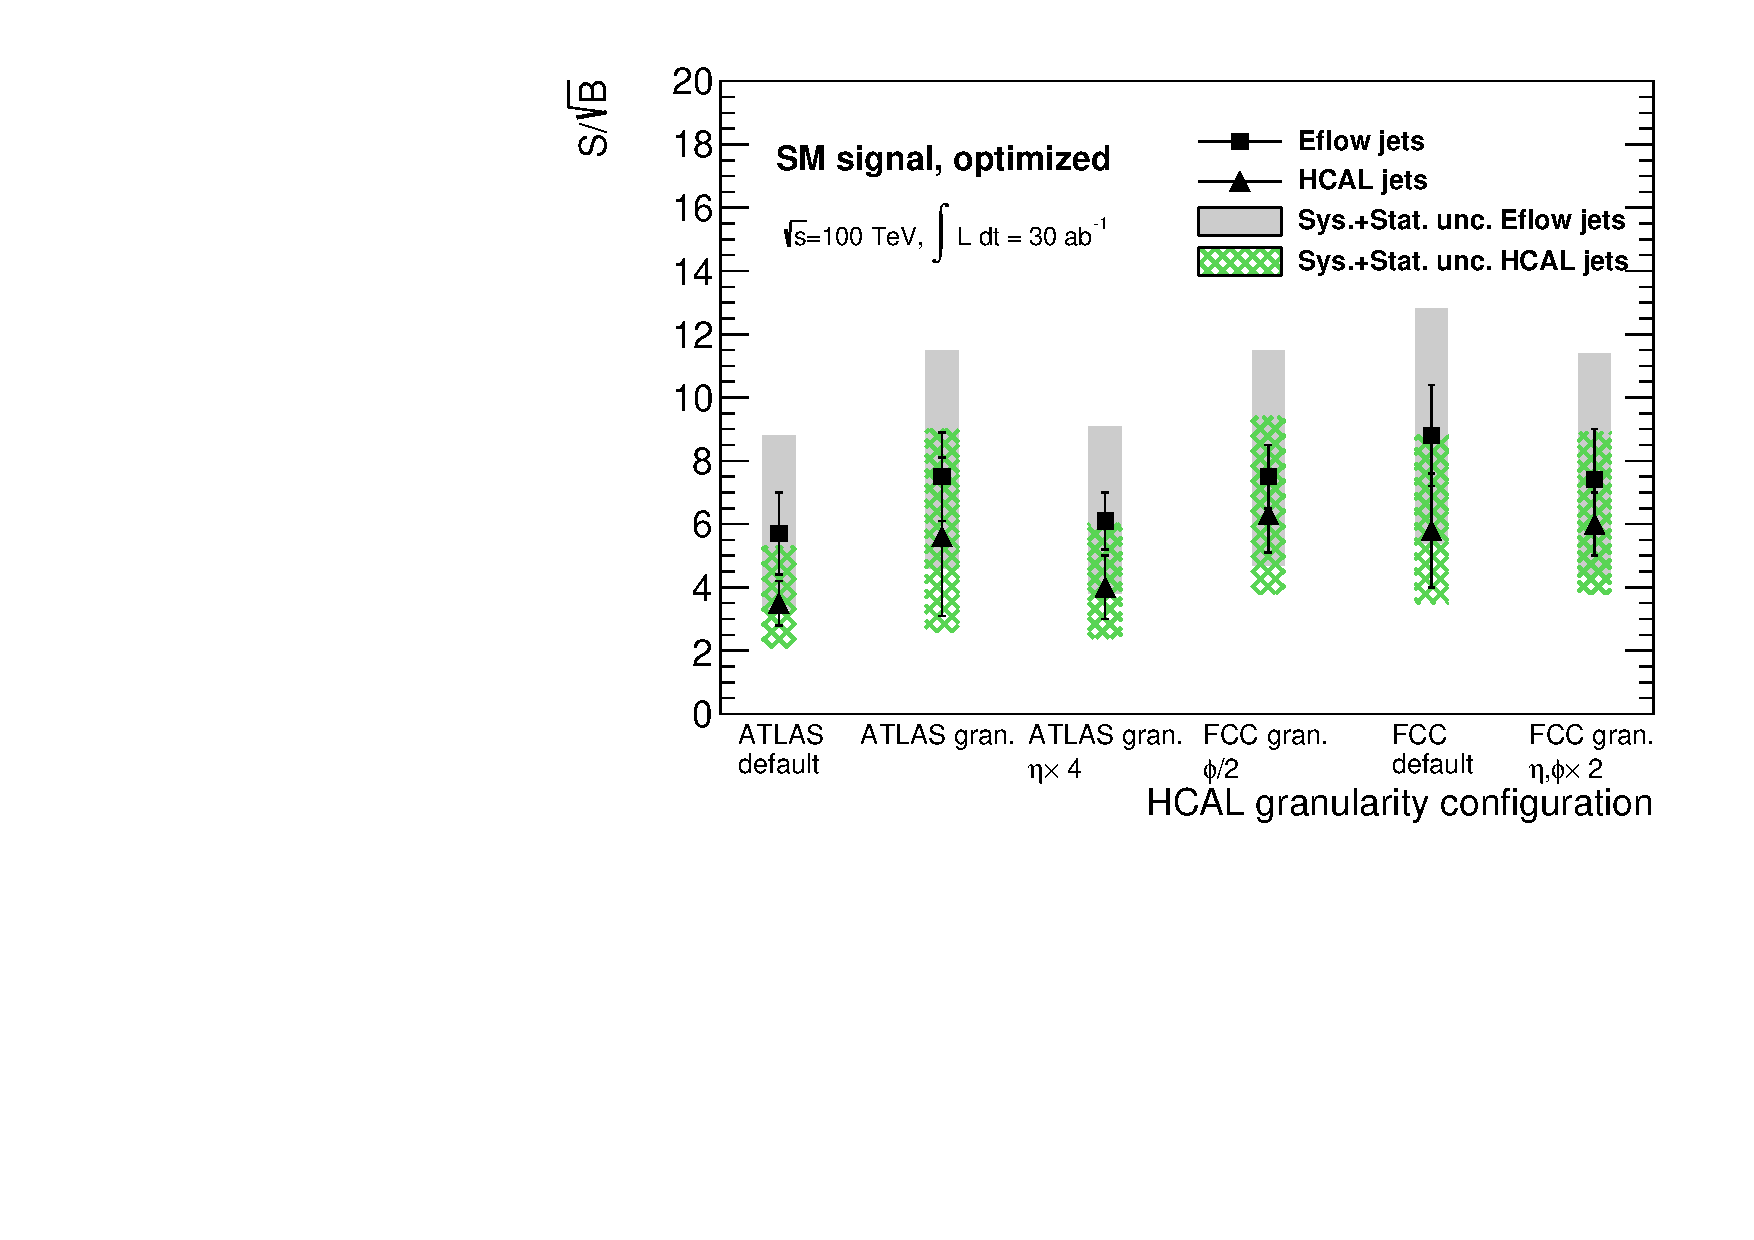
\includegraphics[trim={0 0 .6cm 0},clip,width=\linewidth]{./Figures/SSBvsGran_SM_Opt.pdf}
	\end{minipage}
	\begin{minipage}[t]{0.5\textwidth}
		\caption*{(a)}
		%\label{fig1}
	\end{minipage}%%%
	\hfill
	\begin{minipage}[t]{0.5\textwidth}
		\caption*{(b)}
		%\label{fig2}
	\end{minipage}
	\caption{Significance as a function of the detector configuration for the SM signal, for the baseline (a) and optimized (b) analyses. The significances are shown for eflow jets (squares) and pure HCAL jets (triangles).}
	\label{fig:SSBvsGran1}
\end{figure}

\begin{figure}
	\centering
	\begin{minipage}{.5\textwidth}
		\centering
		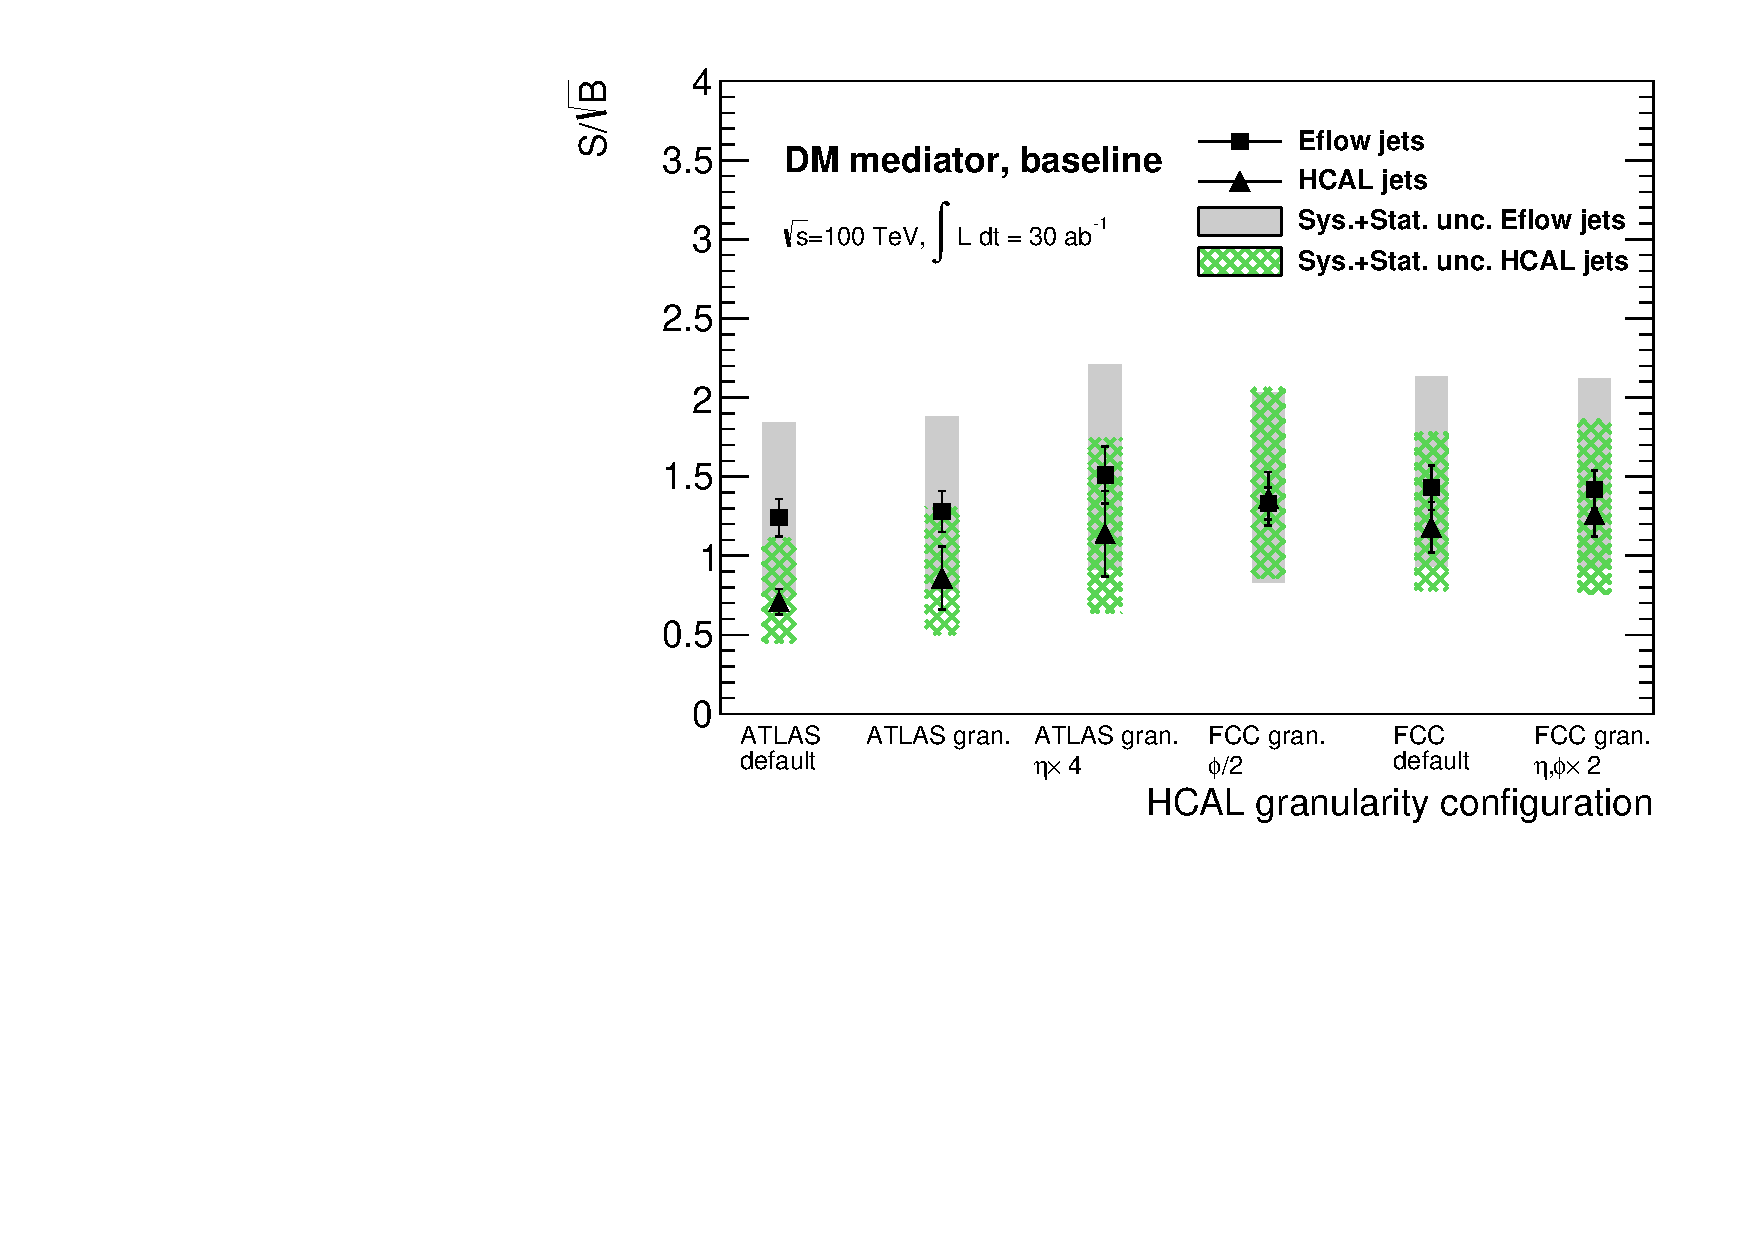
\includegraphics[trim={.6cm 0 0 0},clip,width=\linewidth]{./Figures/SSBvsGran_DM.pdf}
	\end{minipage}%
	\begin{minipage}{.5\textwidth}
		\centering
		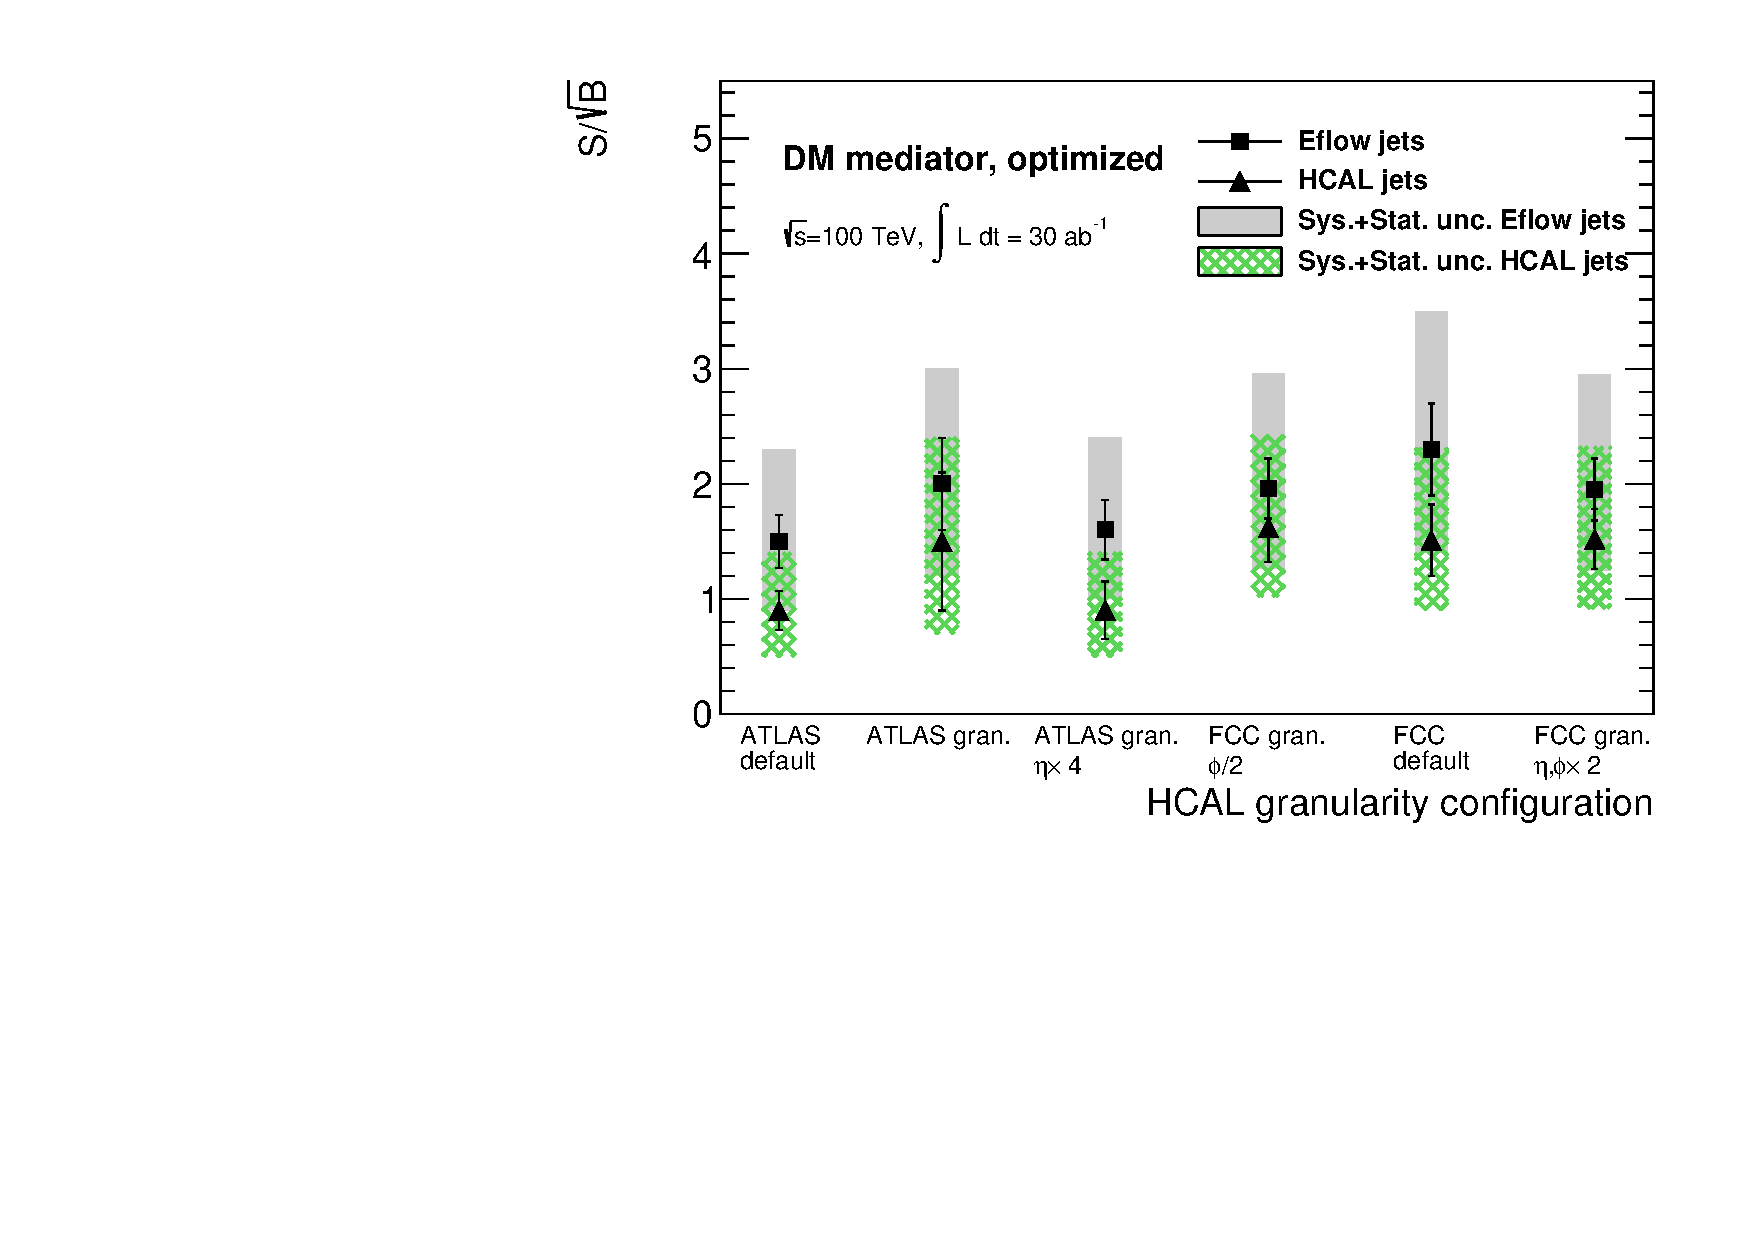
\includegraphics[trim={0 0 .6cm 0},clip,width=\linewidth]{./Figures/SSBvsGran_DM_Opt.pdf}
	\end{minipage}
	\begin{minipage}[t]{0.5\textwidth}
		\caption*{(a)}
		%\label{fig1}
	\end{minipage}%%%
	\hfill
	\begin{minipage}[t]{0.5\textwidth}
		\caption*{(b)}
		%\label{fig2}
	\end{minipage}
	\caption{Significance as a function of the detector configuration for the DM mediator signal, for the baseline (a) and optimized (b) analyses. The significances are shown for eflow jets (squares) and pure HCAL jets (triangles).}
	\label{fig:SSBvsGran2}
\end{figure}

\begin{figure}
	\centering
	\begin{minipage}{.5\textwidth}
		\centering
		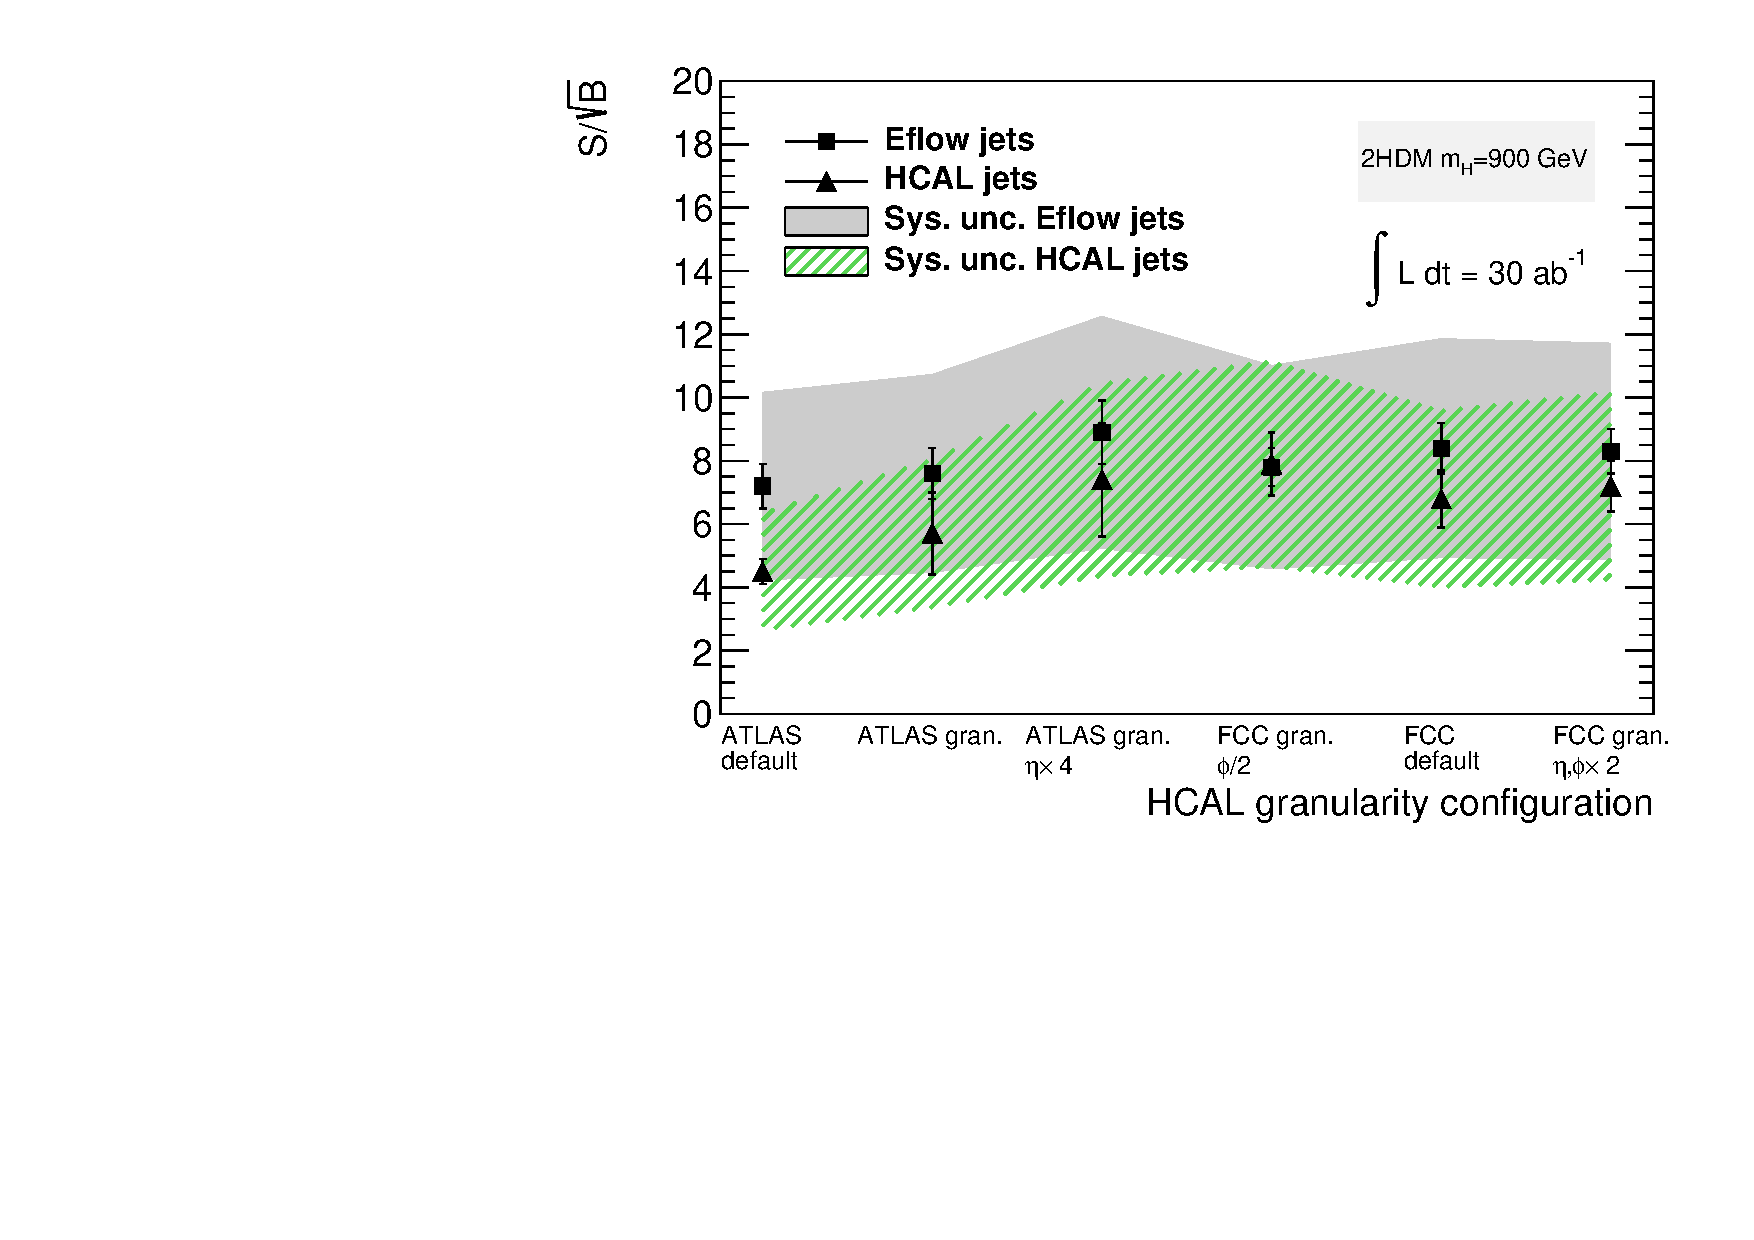
\includegraphics[trim={.6cm 0 0 0},clip,width=\linewidth]{./Figures/SSBvsGran_2HDM.pdf}
	\end{minipage}%
	\begin{minipage}{.5\textwidth}
		\centering
		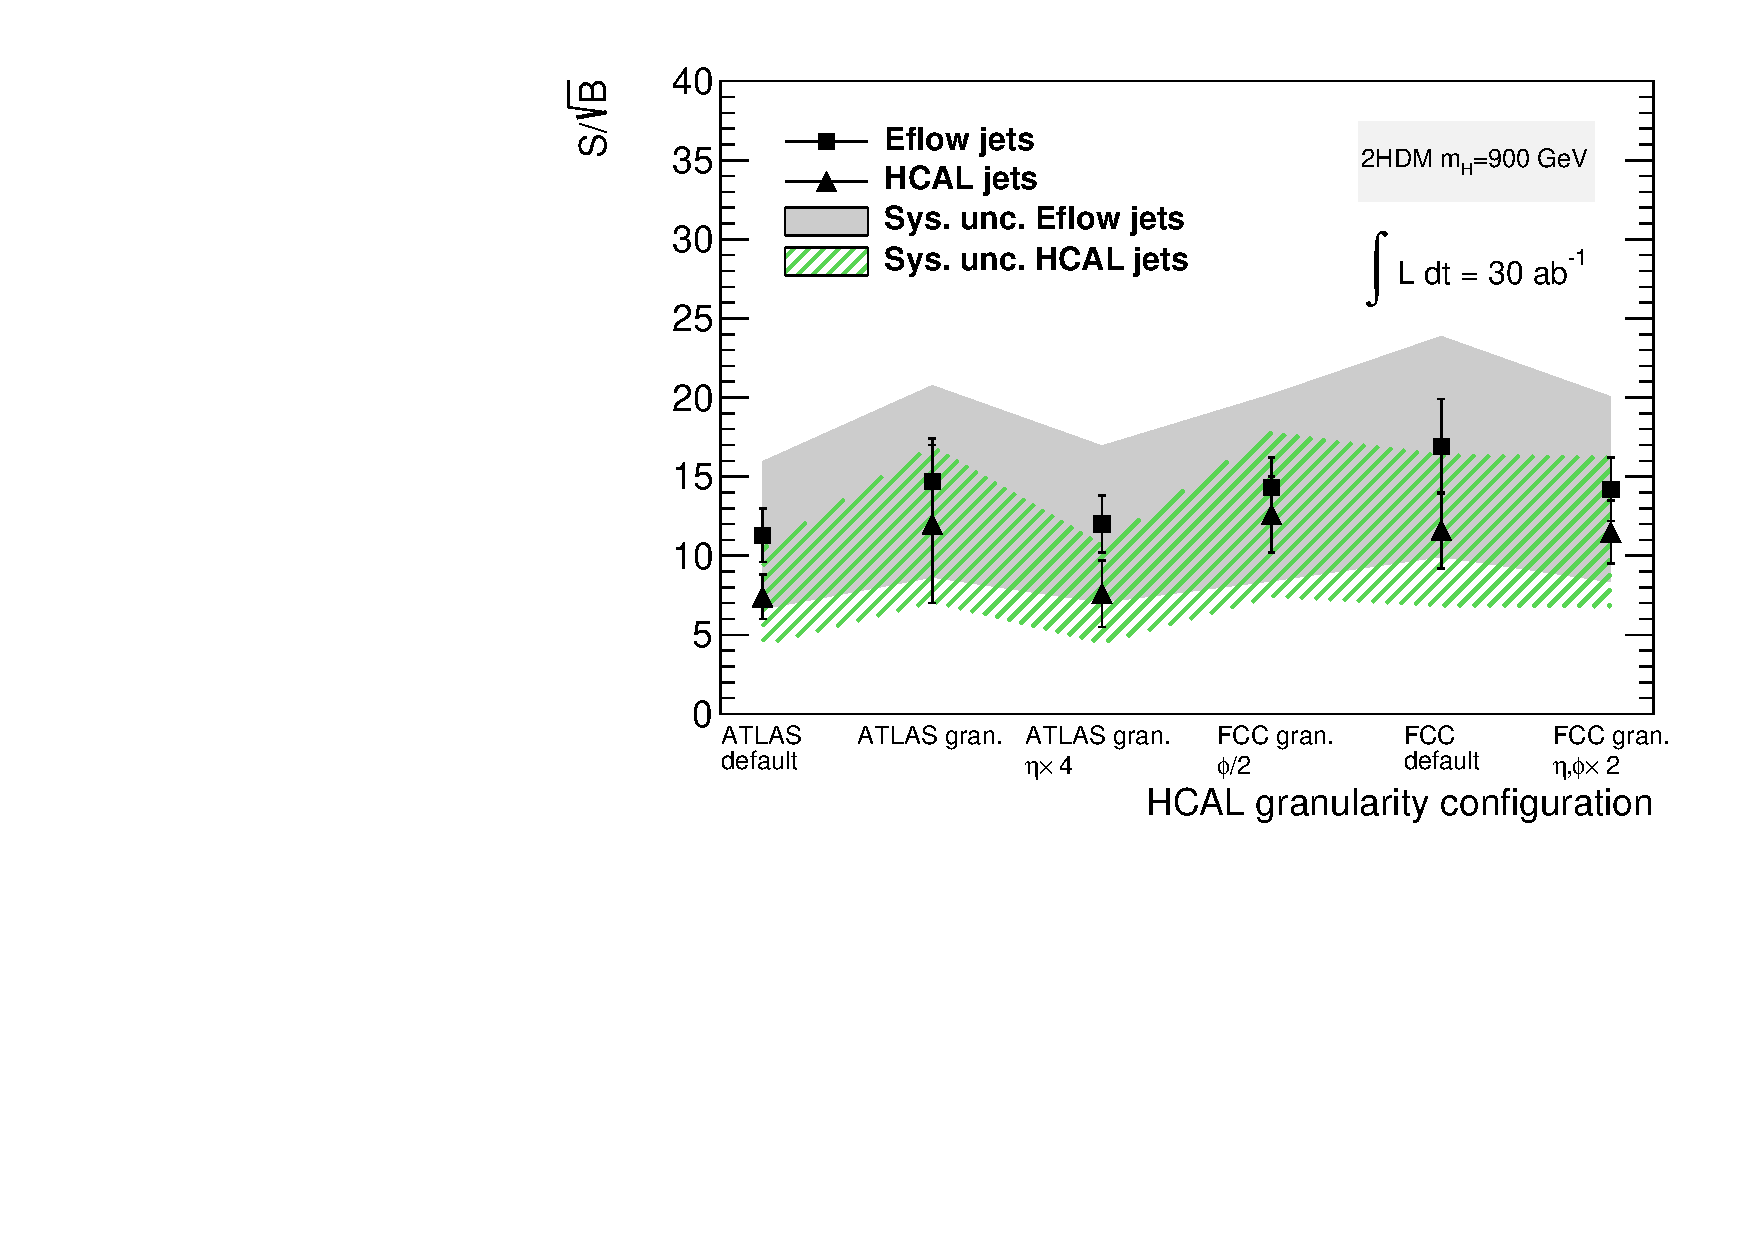
\includegraphics[trim={0 0 .6cm 0},clip,width=\linewidth]{./Figures/SSBvsGran_2HDM_Opt.pdf}
	\end{minipage}
	\begin{minipage}[t]{0.5\textwidth}
		\caption*{(a)}
		%\label{fig1}
	\end{minipage}%%%
	\hfill
	\begin{minipage}[t]{0.5\textwidth}
		\caption*{(b)}
		%\label{fig2}
	\end{minipage}
	\caption{Significance as a function of the detector configuration for the 2HDM signal, for the baseline (a) and optimized (b) analyses. The significances are shown for eflow jets (squares) and pure HCAL jets (triangles).}
	\label{fig:SSBvsGran3}
\end{figure}

%\begin{figure}
%	\centering
%	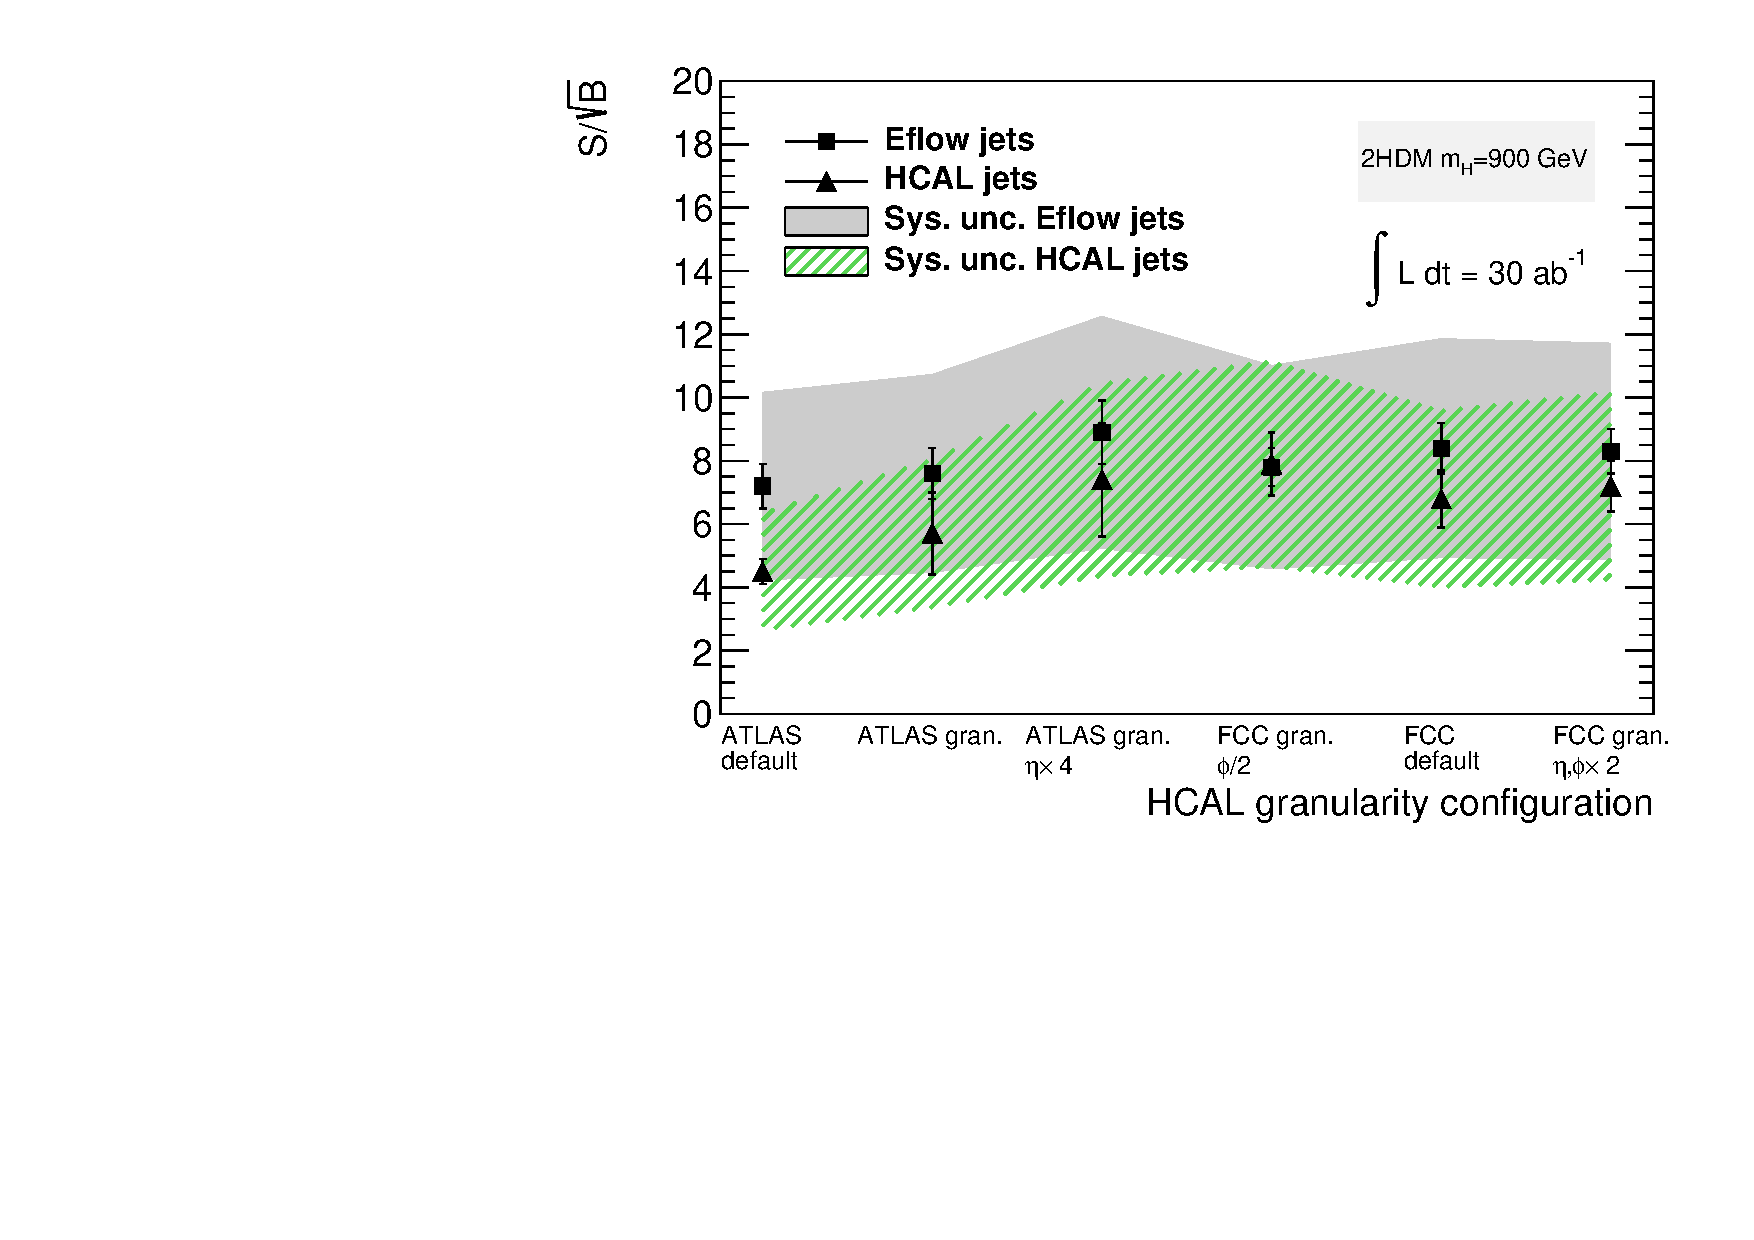
\includegraphics[width=0.5\linewidth]{./Figures/SSBvsGran_2HDM.pdf}
%	\caption{Significance as a function of the detector configuration for the 2HDM with $m_H=900$ GeV. The significances are shown for $\mathcal{L}=30~\text{ab}^{-1}$ (filled) and $\mathcal{L}=3~\text{ab}^{-1}$ (empty) and for particle flow jets (squares) and pure calorimeter (HCAL) jets (triangles).}
%	\label{fig:SSBvsGran_2HDM}
%\end{figure}

%\begin{figure}[!htb]
%  \centering
%  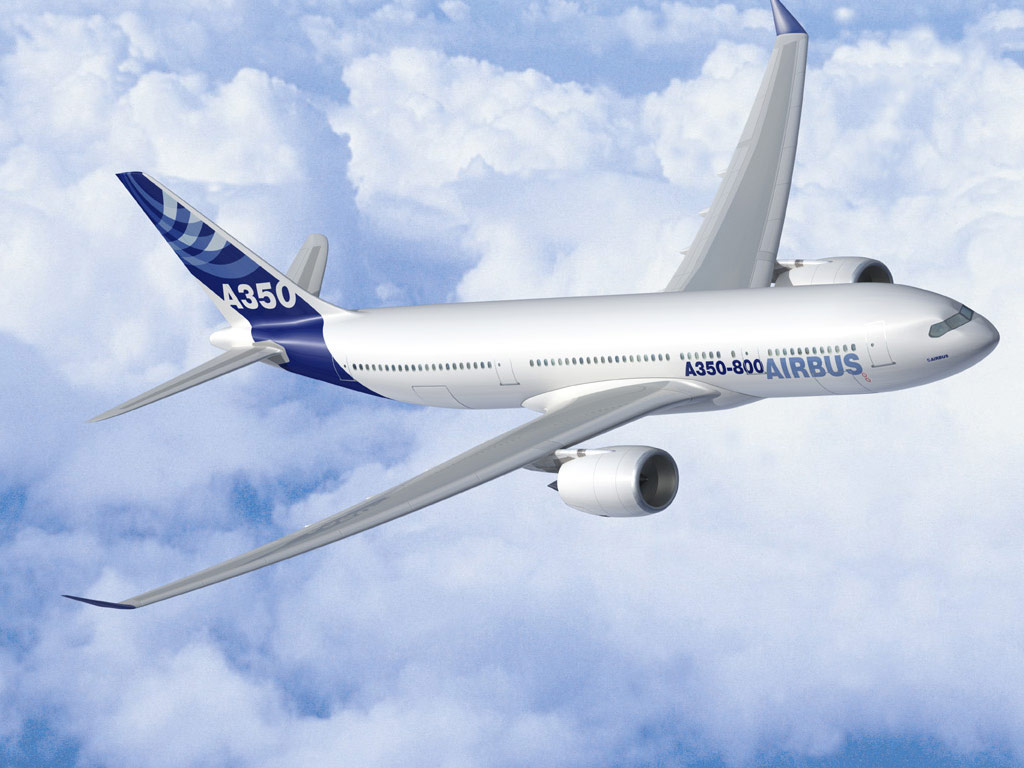
\includegraphics[width=0.25\textwidth]{Figures/Airbus_A350.jpg}
%  \caption[Caption for figure in TOC.]{Caption for figure.}
%  \label{fig:airbus1}
%\end{figure}
%
%\begin{figure}[!htb]
%  \begin{subfigmatrix}{2}
%    \subfigure[Airbus A320]{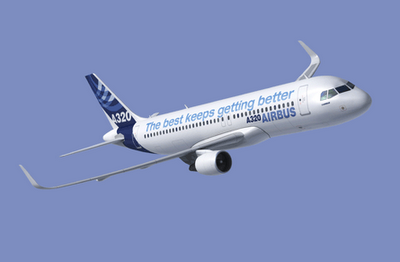
\includegraphics[width=0.49\linewidth]{Figures/Airbus_A320_sharklets.png}}
%    \subfigure[Bombardier CRJ200]{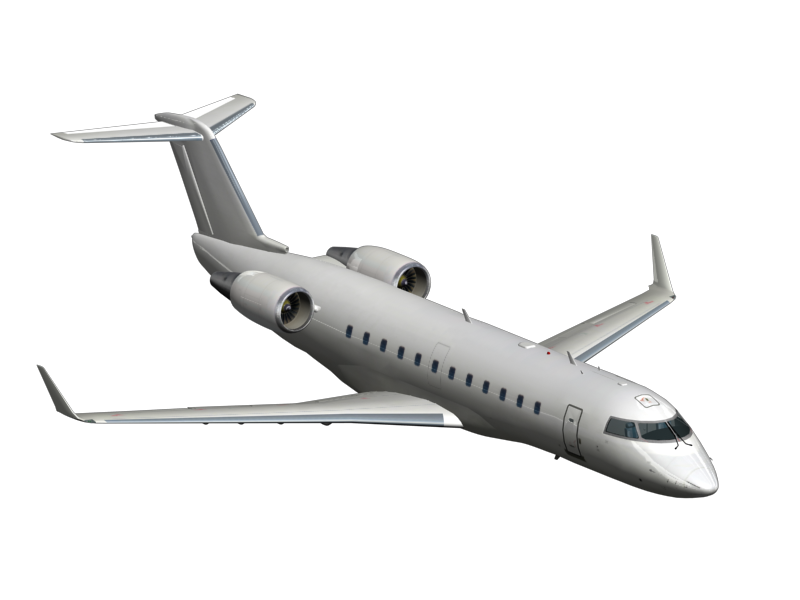
\includegraphics[width=0.49\linewidth]{Figures/Bombardier_CRJ200.png}}
%  \end{subfigmatrix}
%  \caption{Some aircrafts.}
%  \label{fig:aircrafts}
%\end{figure}
%
%Make reference to Figures \ref{fig:airbus1} and \ref{fig:aircrafts}.
%
%By default, the supported file types are {\it .png,.pdf,.jpg,.mps,.jpeg,.PNG,.PDF,.JPG,.JPEG}.
%
%See \url{http://mactex-wiki.tug.org/wiki/index.php/Graphics_inclusion} for adding support to other extensions.
%
%
%% ----------------------------------------------------------------------
%\subsubsection{Drawings}
%\label{subsection:drawings}
%
%Insert your subsection material and for instance a few drawings...
%
%The schematic illustrated in Fig.~\ref{fig:algorithm} can represent some sort of algorithm.
%
%\begin{figure}[!htb]
%  \centering
%  \scriptsize
%%  \footnotesize 
%%  \small
%  \setlength{\unitlength}{0.9cm}
%  \begin{picture}(8.5,6)
%    \linethickness{0.3mm}
%
%    \put(3,6){\vector(0,-1){1}}
%    \put(3.5,5.4){$\bf \alpha$}
%    \put(3,4.5){\oval(6,1){}}
%    %\put(0,4){\framebox(6,1){}}
%    \put(0.3,4.4){Grid Generation: \quad ${\bf x} = {\bf x}\left({\bf \alpha}\right)$}
%
%    \put(3,4){\vector(0,-1){1}}
%    \put(3.5,3.4){$\bf x$}
%    \put(3,2.5){\oval(6,1){}}
%    %\put(0,2){\framebox(6,1){}}
%    \put(0.3,2.4){Flow Solver: \quad ${\cal R}\left({\bf x},{\bf q}\left({\bf x}\right)\right) = 0$}
%
%    \put(6.0,2.5){\vector(1,0){1}}
%    \put(6.4,3){$Y_1$}
%
%    \put(3,2){\vector(0,-1){1}}
%    \put(3.5,1.4){$\bf q$}
%    \put(3,0.5){\oval(6,1){}}
%    %\put(0,0){\framebox(6,1){}}
%    \put(0.3,0.4){Structural Solver: \quad ${\cal M}\left({\bf x},{\bf q}\left({\bf x}\right)\right) = 0$}
%
%    \put(6.0,0.5){\vector(1,0){1}}
%    \put(6.4,1){$Y_2$}
%
%    %\put(7.8,2.5){\oval(1.6,5){}}
%    \put(7.0,0){\framebox(1.6,5){}}
%    \put(7.1,2.5){Optimizer}
%    \put(7.8,5){\line(0,1){1}}
%    \put(7.8,6){\line(-1,0){4.8}}
%  \end{picture}
%  \caption{Schematic of some algorithm.}
%  \label{fig:algorithm}
%\end{figure}
%
%
%% ----------------------------------------------------------------------
%\subsection{Equations}
%\label{subsection:equations}
%
%Equations can be inserted in different ways.
%
%The simplest way is in a separate line like this
%
%\begin{equation}
%  \frac{{\rm d} q_{ijk}}{{\rm d} t} + {\cal R}_{ijk}({\bf q}) = 0 \,.
%\label{eq:ode}
%\end{equation}
%
%If the equation is to be embedded in the text. One can do it like this ${\partial {\cal R}}/{\partial {\bf q}}=0$.
%
%It may also be split in different lines like this
%
%\begin{eqnarray}
%  {\rm Minimize}   && Y({\bf \alpha},{\bf q}({\bf \alpha}))            \nonumber           \\
%  {\rm w.r.t.}     && {\bf \alpha} \,,                                 \label{eq:minimize} \\
%  {\rm subject~to} && {\cal R}({\bf \alpha},{\bf q}({\bf \alpha})) = 0 \nonumber           \\
%                   &&       C ({\bf \alpha},{\bf q}({\bf \alpha})) = 0 \,. \nonumber
%\end{eqnarray}
%
%It is also possible to use subequations. Equations~\ref{eq:continuity}, \ref{eq:momentum} and \ref{eq:energy} form the Naver--Stokes equations~\ref{eq:NavierStokes}.
%
%\begin{subequations}
%    \begin{equation}
%    \frac{\partial \rho}{\partial t} + \frac{\partial}{\partial x_j}\left( \rho u_j \right) = 0 \,,
%    \label{eq:continuity}
%    \end{equation}
%    \begin{equation}
%    \frac{\partial}{\partial t}\left( \rho u_i \right) + \frac{\partial}{\partial x_j} \left( \rho u_i u_j + p \delta_{ij} - \tau_{ji} \right) = 0, \quad i=1,2,3 \,,
%    \label{eq:momentum}
%    \end{equation}
%    \begin{equation}
%        \frac{\partial}{\partial t}\left( \rho E \right) + \frac{\partial}{\partial x_j} \left( \rho E u_j + p u_j - u_i \tau_{ij} + q_j \right) = 0 \,.
%    \label{eq:energy}
%    \end{equation}
%\label{eq:NavierStokes}%
%\end{subequations}
%
%
%% ----------------------------------------------------------------------
%\subsection{Tables}
%\label{section:tables}
%
%Insert your subsection material and for instance a few tables...
%
%Make sure all tables presented are referenced in the text!
%
%Follow some guidelines when making tables:
%
%\begin{itemize}
%  \item Avoid vertical lines
%  \item Avoid “boxing up” cells, usually 3 horizontal lines are enough: above, below, and after heading
%  \item Avoid double horizontal lines
%  \item Add enough space between rows
%\end{itemize}
%
%\begin{table}[!htb]
%  \renewcommand{\arraystretch}{1.2} % more space between rows
%  \centering
%  \begin{tabular}{lccc}
%    \toprule
%    Model           & $C_L$ & $C_D$ & $C_{M y}$ \\
%    \midrule
%    Euler           & 0.083 & 0.021 & -0.110    \\
%    Navier--Stokes  & 0.078 & 0.023 & -0.101    \\
%    \bottomrule
%  \end{tabular}
%  \caption[Table caption shown in TOC.]{Table caption.}
%  \label{tab:aeroCoeff}
%\end{table}
%
%Make reference to Table \ref{tab:aeroCoeff}.
%
%Tables \ref{tab:memory} and \ref{tab:multipleColumns} are examples of tables with merging columns:
%
%\begin{table}[!htb]
%  \renewcommand{\arraystretch}{1.2} % more space between rows
%  \centering
%  \begin{tabular}[]{lrr}
%    \toprule
%                & \multicolumn{2}{c}{\underline{Virtual memory [MB]}} \\
%                & Euler       & Navier--Stokes \\
%    \midrule
%      Wing only &  1,000      &    2,000       \\
%      Aircraft  &  5,000      &   10,000       \\
%      (ratio)   & $5.0\times$ & $5.0\times$    \\
%    \bottomrule
%  \end{tabular}
%  \caption{Memory usage comparison (in MB).}
%  \label{tab:memory}
%\end{table}
%
%\begin{table}[!htb]
%  \centering
%  \renewcommand{\arraystretch}{1.2} % more space between rows
%  \begin{tabular}{@{}rrrrcrrr@{}} % remove space to the vertical edges @{}...@{}
%    \toprule
%      & \multicolumn{3}{c}{$w = 2$} & \phantom{abc} & \multicolumn{3}{c}{$w = 4$} \\
%    \cmidrule{2-4}
%    \cmidrule{6-8}
%      & $t=0$ & $t=1$ & $t=2$ && $t=0$ & $t=1$ & $t=2$ \\
%    \midrule
%      $dir=1$
%      \\
%      $c$ &  0.07 &  0.16 &  0.29 &&  0.36 &  0.71 &   3.18 \\
%      $c$ & -0.86 & 50.04 &  5.93 && -9.07 & 29.09 &  46.21 \\
%      $c$ & 14.27 &-50.96 &-14.27 && 12.22 &-63.54 &-381.09 \\
%      $dir=0$
%      \\
%      $c$ &  0.03 &  1.24 &  0.21 &&  0.35 & -0.27 &  2.14 \\
%      $c$ &-17.90 &-37.11 &  8.85 &&-30.73 & -9.59 & -3.00 \\
%      $c$ &105.55 & 23.11 &-94.73 &&100.24 & 41.27 &-25.73 \\
%    \bottomrule
%  \end{tabular}
%  \caption{Another table caption.}
%  \label{tab:multipleColumns}
%\end{table}
%
%An example with merging rows can be seen in Tab.\ref{tab:multipleRows}.
%
%\begin{table}[!htb]
%  \renewcommand{\arraystretch}{1.2} % more space between rows
%  \centering
%  \begin{tabular}{ccccc}
%    \toprule
%      \multirow{2}{*}{ABC} & \multicolumn{4}{c}{header} \\
%      \cmidrule{2-5} & 1.1 & 2.2 & 3.3 & 4.4 \\
%    \midrule
%      \multirow{2}{*}{IJK} & \multicolumn{2}{c}{\multirow{2}{*}{group}} & 0.5 & 0.6 \\
%      \cmidrule{4-5}       & \multicolumn{2}{c}{}                       & 0.7 & 1.2 \\
%    \bottomrule
%  \end{tabular}
%  \caption{Yet another table caption.}
%  \label{tab:multipleRows}
%\end{table}
%
%If the table has too many columns, it can be scaled to fit the text widht, as in Tab.\ref{tab:scale}.
%\begin{table}[!htb]
%  \renewcommand{\arraystretch}{1.2} % more space between rows
%  \centering
%  \resizebox*{\textwidth}{!}{%
%    \begin{tabular}[]{lcccccccccc}
%      \toprule
%        Variable &  a  &  b  &  c  &  d  &  e  &  f  &  g  &  h  &  i  &  j  \\
%      \midrule
%        Test 1   &  10,000 &  20,000 &  30,000 &  40,000 &  50,000 &  60,000 &  70,000 &  80,000 &  90,000 & 100,000 \\
%        Test 2   &  20,000 &  40,000 &  60,000 &  80,000 & 100,000 & 120,000 & 140,000 & 160,000 & 180,000 & 200,000 \\
%      \bottomrule
%    \end{tabular}
%  }%
%  \caption{Very wide table.}
%  \label{tab:scale}%
%\end{table}
%
%
%% ----------------------------------------------------------------------
%\subsection{Mixing}
%\label{section:mixing}
%
%If necessary, a figure and a table can be put side-by-side as in Fig.\ref{fig:side_by_side}
%
%\begin{figure}[!htb]
%  \begin{minipage}[b]{0.60\linewidth}
%    \centering
%    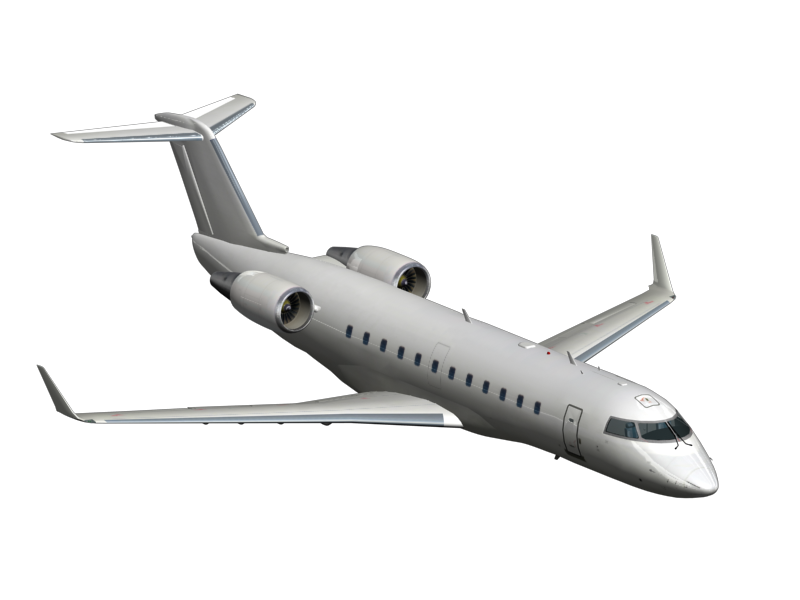
\includegraphics[width=\linewidth]{Figures/Bombardier_CRJ200}
%  \end{minipage}%
%  \begin{minipage}[b]{0.30\linewidth}
%    \centering
%    \begin{tabular}[b]{lll}
%      \toprule
%        \multicolumn{3}{c}{Legend} \\
%      \midrule
%        A & B & C \\
%        0 & 0 & 0 \\
%        0 & 1 & 0 \\
%        1 & 0 & 0 \\
%        1 & 1 & 1 \\
%      \bottomrule
%    \end{tabular}
%    \vspace{5em}
%  \end{minipage}
%\caption{Figure and table side-by-side.}
%\label{fig:side_by_side}
%\end{figure}

